\section{Autonomous landing algorithm}
\label{sec:algo}

The processing pipeline of the algorithm can be broken down into the following main steps.

\subsubsection{Data preprocessing} The algorithm uses high resolution point cloud generated from a mapping system as input. The preprocessing step brings the point cloud into a uniform resolution for analysis.

\subsubsection{Landing area detection}: The conditions for safe landing on the seafloor are identified for detecting a safe landing area within the point cloud. An exclusion zone is also identified where the centre of gravity of the vehicle is prohibited form landing.
 
\subsubsection{Landing site identification} Within the detected landing area, landing sites are identified which are regions where an AUV of a particular geometry can fit along a certain heading. Landing site properties are extracted for all the identified sites along different headings. 

\subsubsection{Final landing site selection} Landing costs are calculated for all the sites using the landing site properties. The site with minimum landing cost is finally selected as the final landing site.

\subsection{Data preprocessing}
\label{sub:mapping}

The algorithm requires high resolution bathymetry point cloud generated from a  mapping system as described in Section~\ref{ssec:hres}. Data was collected at a Manganese crust site on the No.$5$ Takuyo seamount by a similar mapping system mounted on the AUV BOSS-A during KR$16$-$01$ cruise of R/V Keirei, the specifications of which are given in Table.~\ref{t:table1}. Fig.~\ref{sf:mehul4a} shows a $25$ m section of the bathymetry point cloud mapped at an heading of $-130^\circ$ 

\begin{table}[!ht]
\centering
\caption{Properties of the mapping system}
\begin{tabular}{  |p{6cm}  p{4cm}| }
\hline
\textbf{Property} & \textbf{Value}\\ \hline 
Mapping altitude $a$ & $2$ m \\
Baseline between camera and laser $b$ & $1.025$ m\\
Vertical mounting angle of camera $\phi_m$ & $70^\circ$ \\
Horizontal opening angle of camera $\phi_h$ & $60.2^{\circ}$\\
Vertical opening angle of camera $\phi_v$ & $50.4^{\circ}$\\
Along-track resolution & $4$ mm\\
Cross-track resolution & $3$ mm\\
Vertical resolution & $6$ mm\\

\hline
\end{tabular}
\label{t:table1}
\end{table}

\begin{figure}[!ht]
\centering
\subfloat[Top view of seafloor color reconstruction and depth map. Black rectangles indicate areas where detailed implementation of the algorithm is shown\label{sf:mehul4a}]{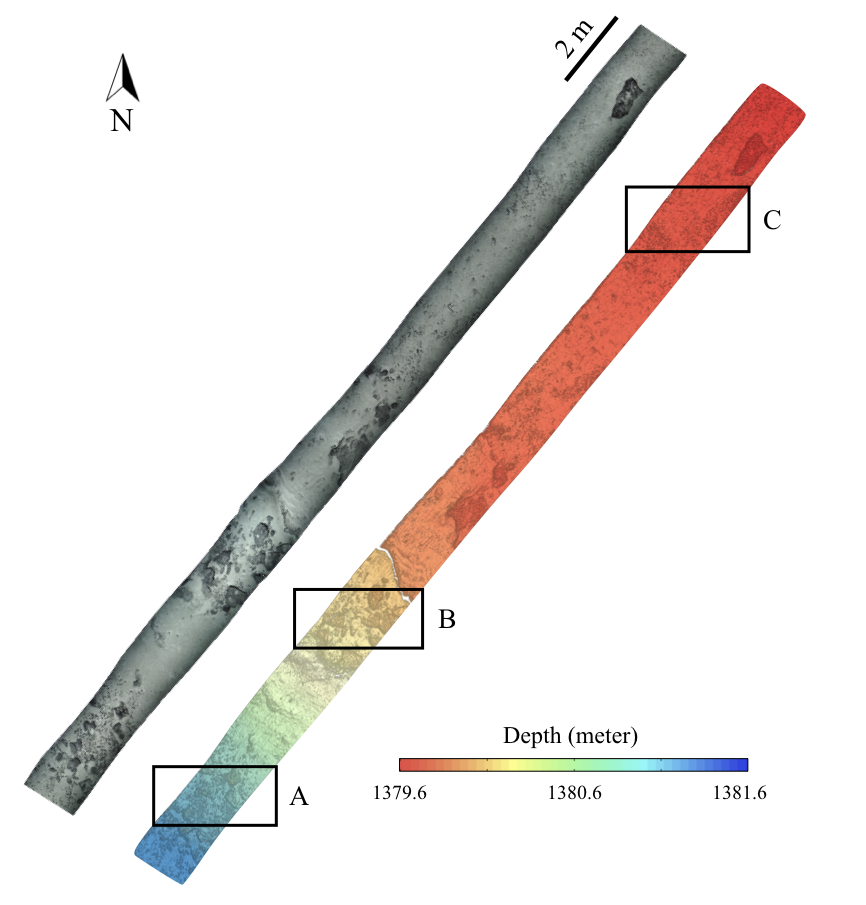
\includegraphics[width=4.5in]{./images/mehul4a.png}}\quad
\subfloat[Resampled point cloud for the three areas A,B and C\label{sf:mehul4b}]{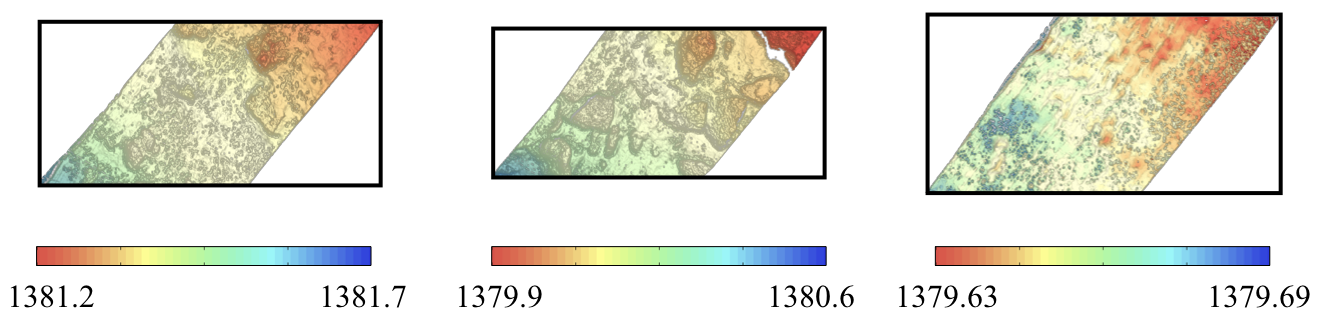
\includegraphics[width=5in]{./images/mehul4b.png}}
\caption{Seafloor bathymetry mapped using high resolution mapping system}
\end{figure}

The mapping system generates the bathymetry point cloud as northing, easting and depth. The point cloud generated from the high resolution mapping system is unstructured and resampled to a uniform grid resolution $g_{res}$. The points resampled with a resolution of $10$ mm are seen in Fig.~\ref{sf:mehul4b}. 

\subsection{Landing area detection}
\label{sub:landingarea}

Conditions for safe landing on the seafloor are determined to identify landing area in the high resolution mapped bathymetry. Landing on sloping surfaces is analyzed for the effects from the righting moment of the AUV, ground friction and seafloor currents. Analysis for safe landing on objects on the seafloor is made considering their heights. In this work, we propose the design on an AUV with negative buoyancy. AUVs are designed and navigate with their centre of buoyancy $C_B$ vertically above the centre of gravity $C_G$.  The key parameters to judge the safety of landing are given in Table~\ref{t:table2} and are defined in Fig.~\ref{f:mehul5}. The table also shows the parameter values used in the simulation of the landing algorithm.
 
\begin{table}[!ht]
\centering
\caption{Physical properties of underwater platform}
\begin{tabular}{ | p{4cm}  p{6cm} p{4cm} | }
\hline
\textbf{Property} & \textbf{Description} & \textbf{Value}\\ \hline 
$l_u$ & length of landing AUV & $1.7$ m\\
$b_u$ & width of landing AUV & $0.5$ m\\
$h_u$ & height of landing AUV & $0.45$ m\\
$F_G$ & force of  gravity (for $65$ Kg mass) & $637$ N \\
$F_B$ & force of buoyancy (for $62$ Kg mass) & $608$ N \\
$F_R$ & net  downward force  & $29$ N \\
$d_g$ & vertical distance to $C_G$ & $0.25$ m \\
$d_m$ & vertical distance between $C_G$ and $C_B$ & $0.05$ m \\
\hline
\end{tabular}
\label{t:table2}
\end{table}

\begin{figure}[!ht]
\centering
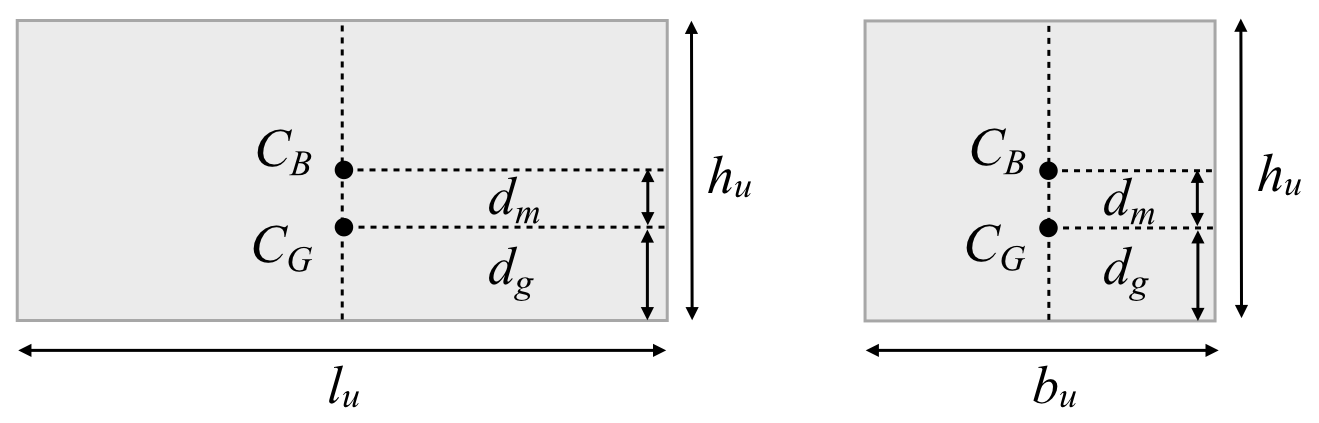
\includegraphics[width=5.0in]{./images/mehul5.png}
\caption{Side and top view of an AUV with parameters used to determine landing conditions}
\label{f:mehul5}
\end{figure}


\subsubsection{Landing on sloping surface}

When landing on a sloping surface, the AUV is considered safe when it can remain stationary and in full contact with the slope. In this work, we determine the minimum slope of the surface for the geometry of the AUV where it can meet this condition. The landing of the AUV on surface with slope is analyzed along different landing orientations of the AUV$\psi$ to find this minimum slope  $\theta_c$ as seen in Fig~\ref{f:mehul6}. 
	While landing, the AUV first makes contact with the slope along its smaller 
	edge $b_u$ for orientations $0^\circ$ and $90^\circ$ and longer edge $l_u$ 
	for orientations $180^\circ$ and $270^\circ$. For all other orientations, 
	the AUV makes contact along one of its corners.

\begin{figure}[!ht]
\centering
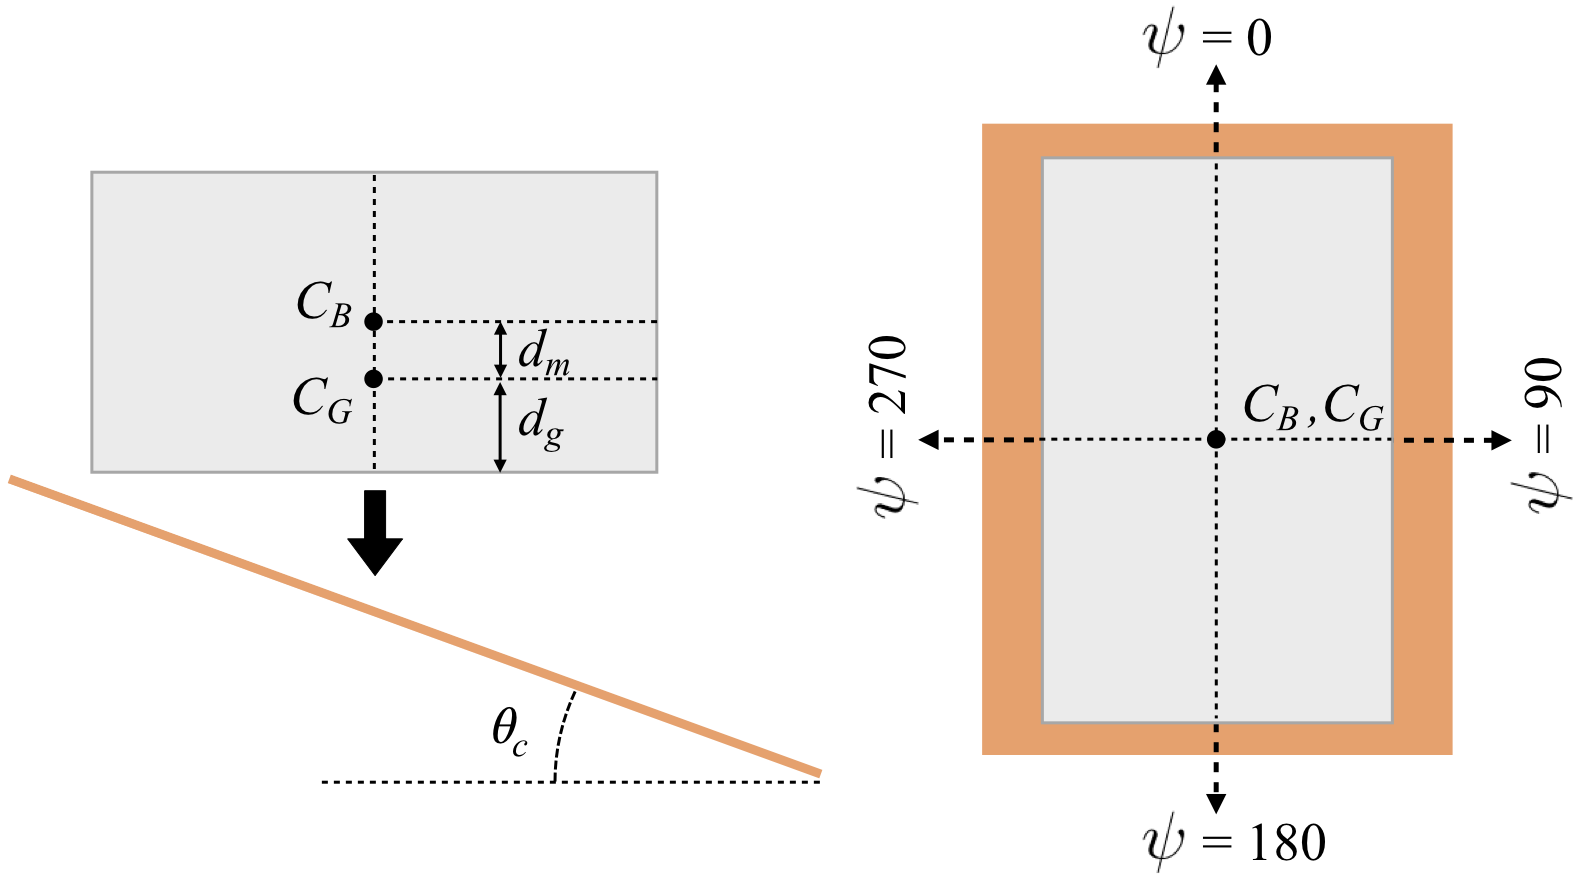
\includegraphics[width=5in]{./images/mehul6.png}
\caption{Side and top view of an AUV landing on a sloping surface}
\label{f:mehul6}
\end{figure}


\begin{figure}[!ht]
\centering
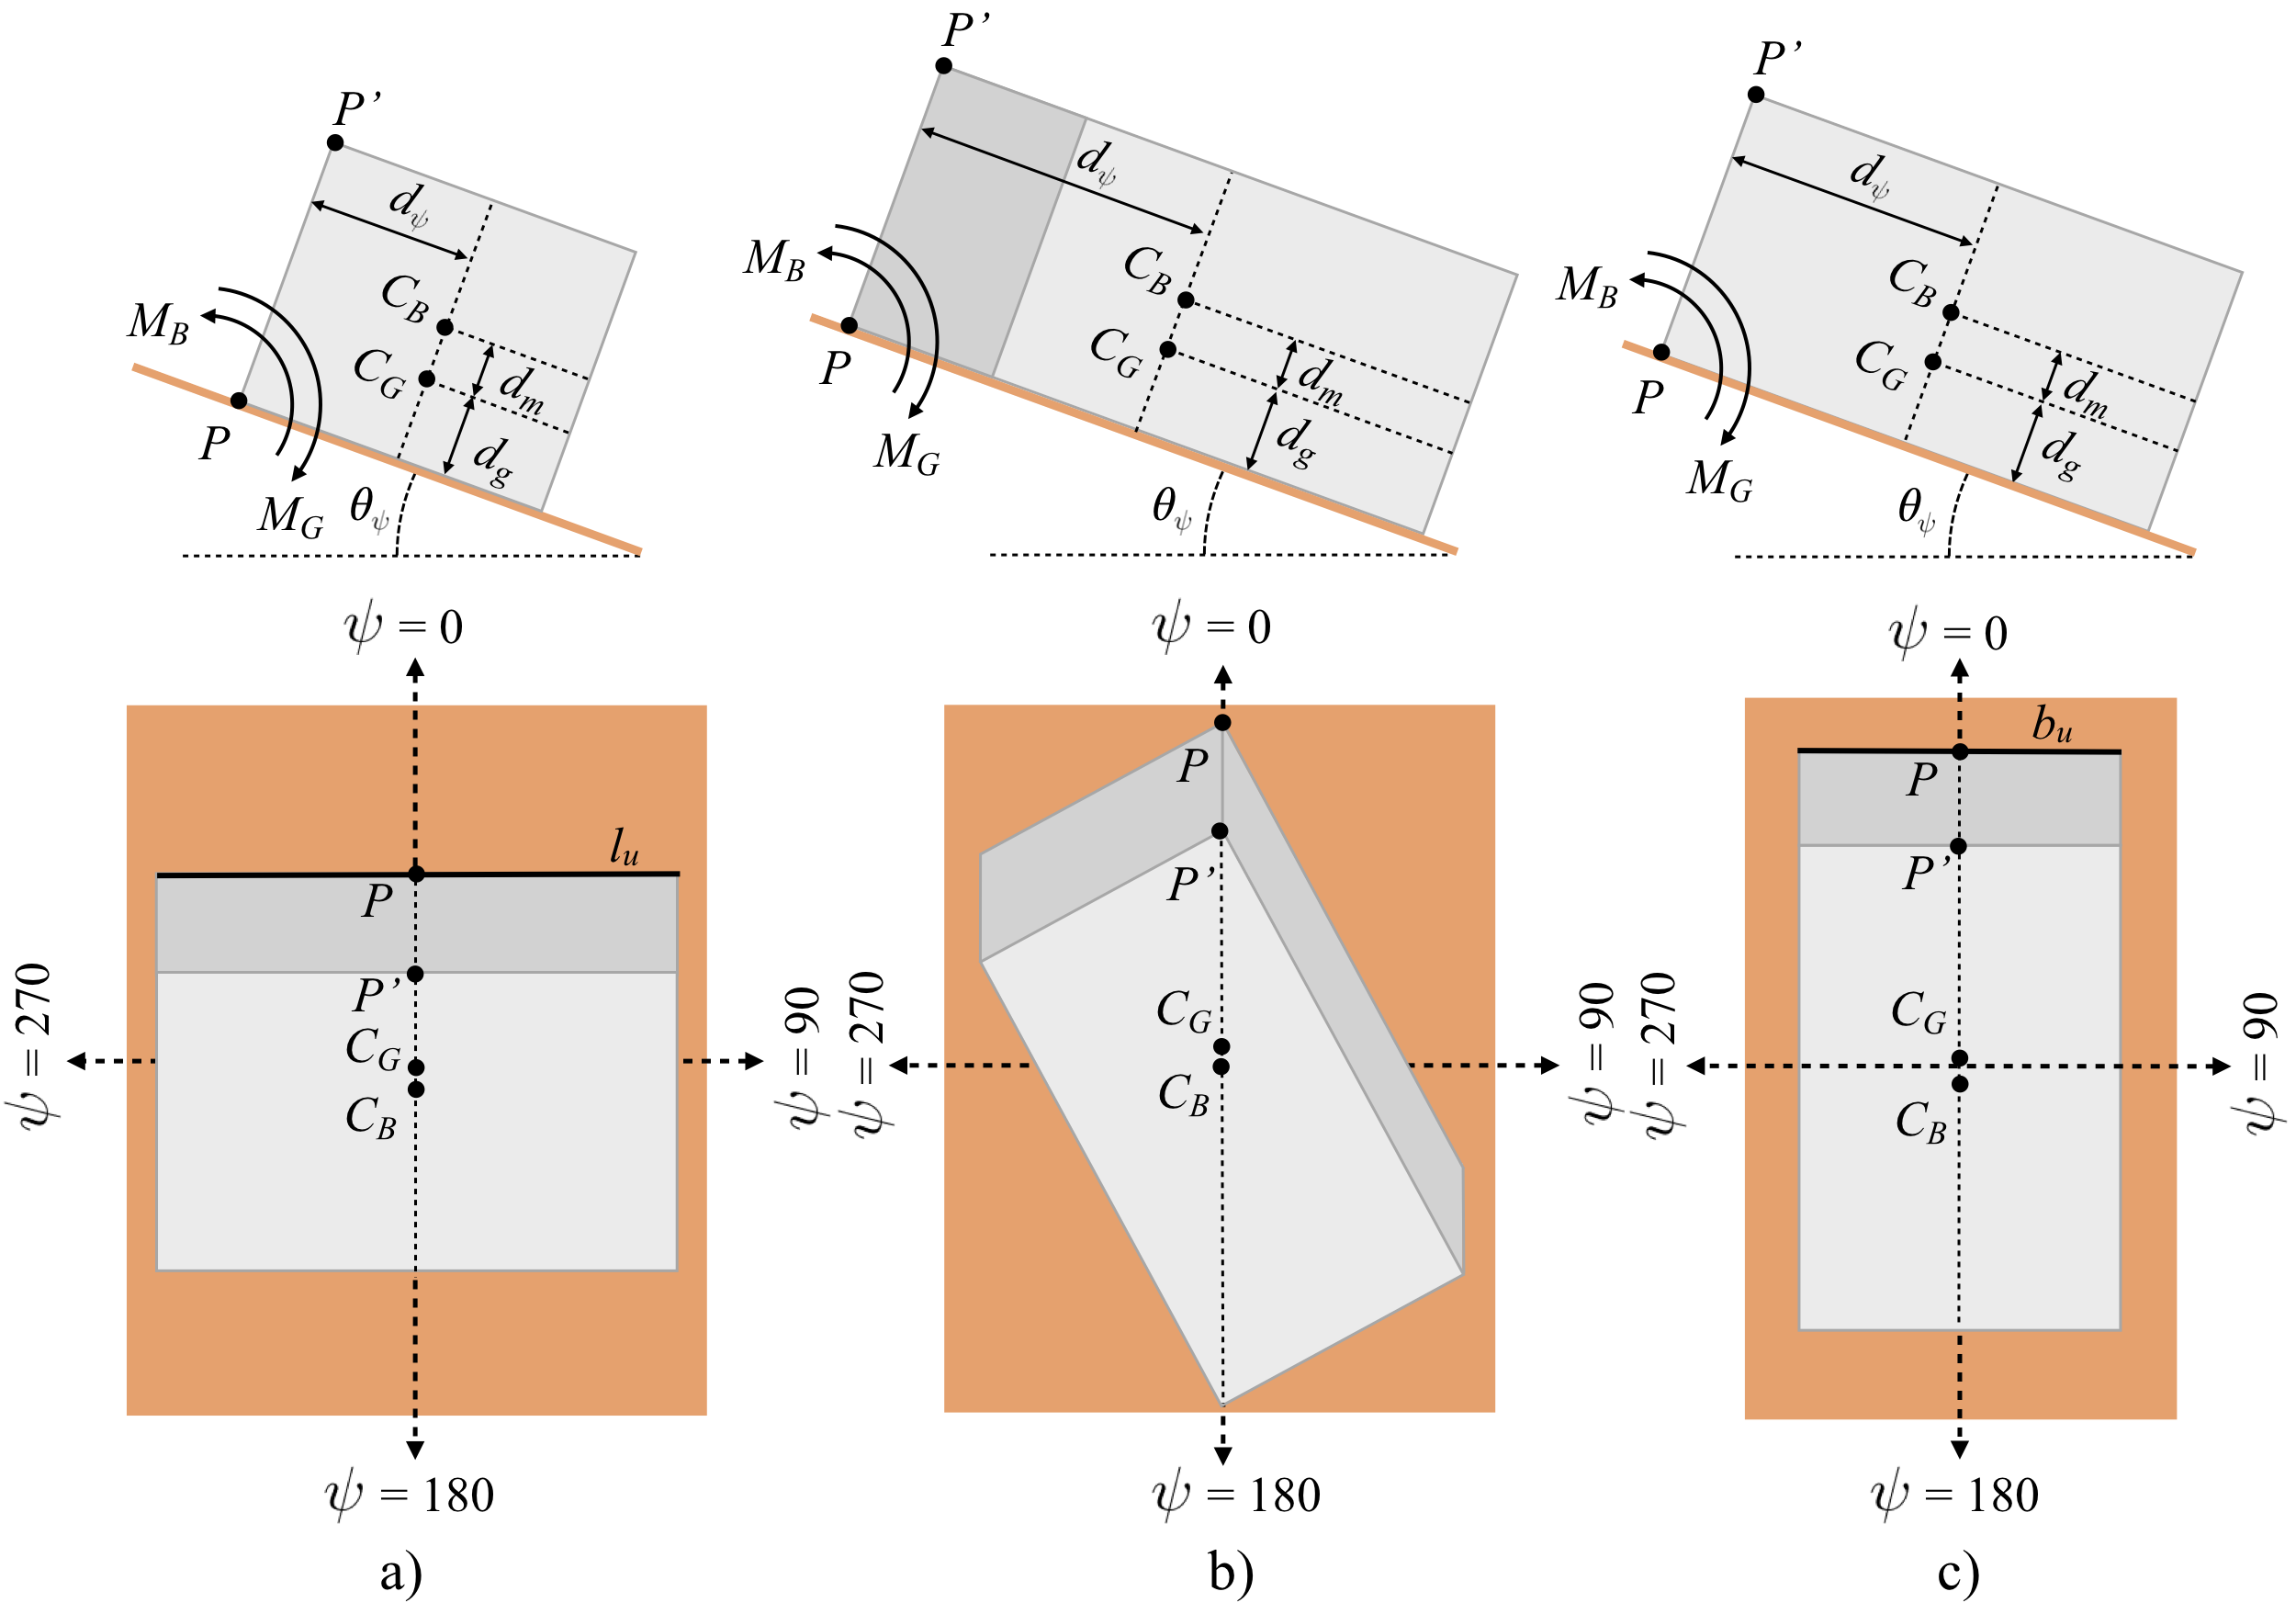
\includegraphics[width=\textwidth]{./images/mehul7.png}
\caption{AUV landing on a sloping surface along different orientations}
\label{f:mehul7}
\end{figure}

After making contact, the AUV can rotate to a maximum angle which is determined by the righting moment of the AUV. The AUV rotates along the plane formed by $C_G$, $C_B$, point $P$ and $P$' as seen in Fig~\ref{f:mehul7}. For a distance $d_{\psi}$ along landing orientation $\psi$, the maximum angle of rotation is given by the equation:

\begin{equation}
\label{eq:eq1}
\centering
	\theta_\psi = \tan^{-1}\left[ \frac{(d_{\psi} \times F_R)}{(d_m \times F_B) - (d_g \times F_R)}\right]
\end{equation}\\

For safe landing, the AUV should make contact with the ground before or at its maximum angle of rotation. While landing along its edges or when normal to the diagonal as seen in Fig~\ref{f:mehul7}, the AUV can make full contact with the surface in one stage. For other orientations, the AUV rotates until one of its edges makes contact with the slope after which it rotates about that edge to make full contact with the surface. The landing of the AUV was simulated along  orientations from $0^\circ$ to  $360^\circ$ to calculate the slope where the AUV can make full contact with the surface for each orientation as seen in Fig~\ref{f:mehul8}. Simulation was also performed for $1$, $2$ and $4$ aspect ratios of $l_u$ and $b_u$ to represent different types of underwater AUVs. From these it was determined that minimum rotation occurs when then AUV lands on its shorter edge $l_u$ as in Fig~\ref{f:mehul7}a resulting in the smallest slope of ground where the AUV can land. The minimum slope of the ground where the AUV can land safely $\theta_c$ is then calculated by using $d_{\psi} = 0.5 \times b_u$ in Equation~\ref{eq:eq1} as follows:

\begin{equation}
\label{eq:eq2}
\centering
	\theta_c = \tan^{-1}\left[ \frac{(0.5 \times b_u \times F_R)}{(d_m \times F_B) - (d_g \times F_R)}\right]
\end{equation}\\


The value of the minimum slope of the ground $\theta_c$ for the simulation using the dimensions of the AUV is calculated as $17.7^\circ$.

\begin{figure}[!ht]
\centering
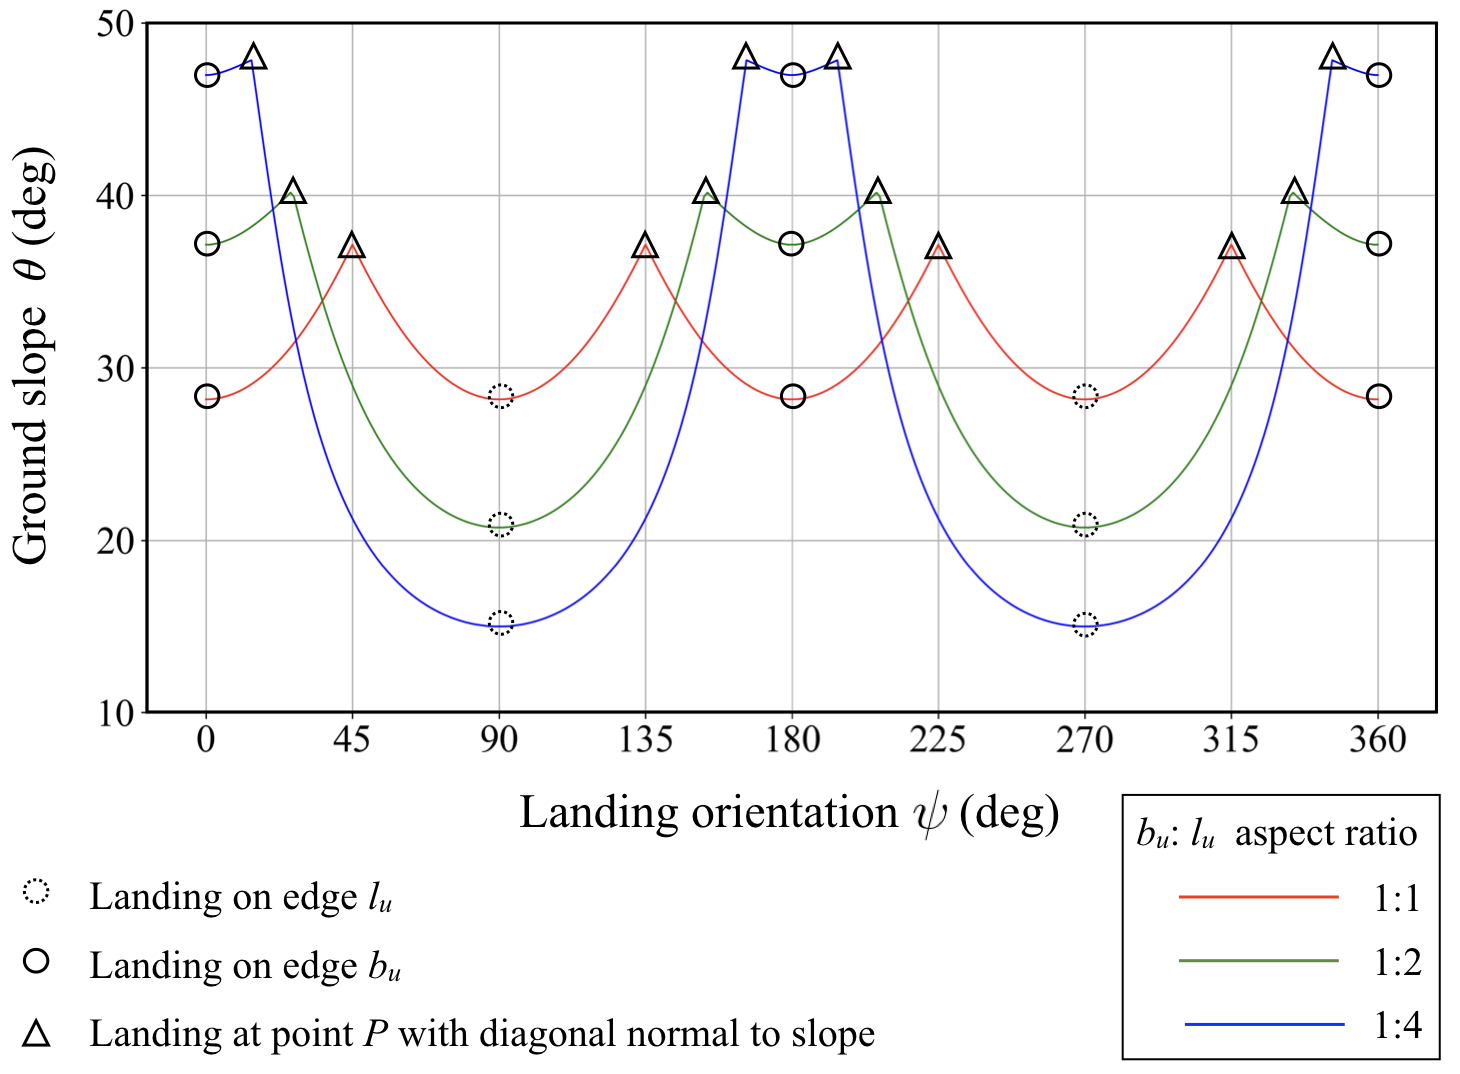
\includegraphics[width=6in]{./images/mehul8.png}
\caption{Slope calculated for different landing orientations and aspect ratios of the AUV}
\label{f:mehul8}
\end{figure}

Once landed, the AUV can remain stationary on the sloping surface if the force of friction $F_F$ counters the component of gravity $F_G$ along the slope and the force due to seafloor currents $F_C$ pushing the vehicle downslope as seen in Fig~\ref{f:mehul9}. The slope of the surface where the vehicle can remain stationary depends on the coefficient of friction $\mu$ between the AUV and seafloor. The relation between the velocity of seafloor currents $v$ and the slope at which the vehicle can remain stationary without slipping  while landing along its longer edge $l_u$ is calculated. For a drag coefficient $C_d = 1.05$ and density $\rho= 1000$ Kg/m$^3$, the velocity of seafloor currents is then calculated as:

\begin{equation}
\label{eq:eq3}
\centering
	Fc = (F_G - F_B) \times (\mu \cos\theta - \sin\theta)
\end{equation}

\begin{equation}
\label{eq:eq4}
\centering
	v_c = \sqrt{ \frac{2 \times Fc}{C_d  \times  \rho  \times  l_u \times h_u}}
\end{equation}


\begin{figure}[!ht]
\centering
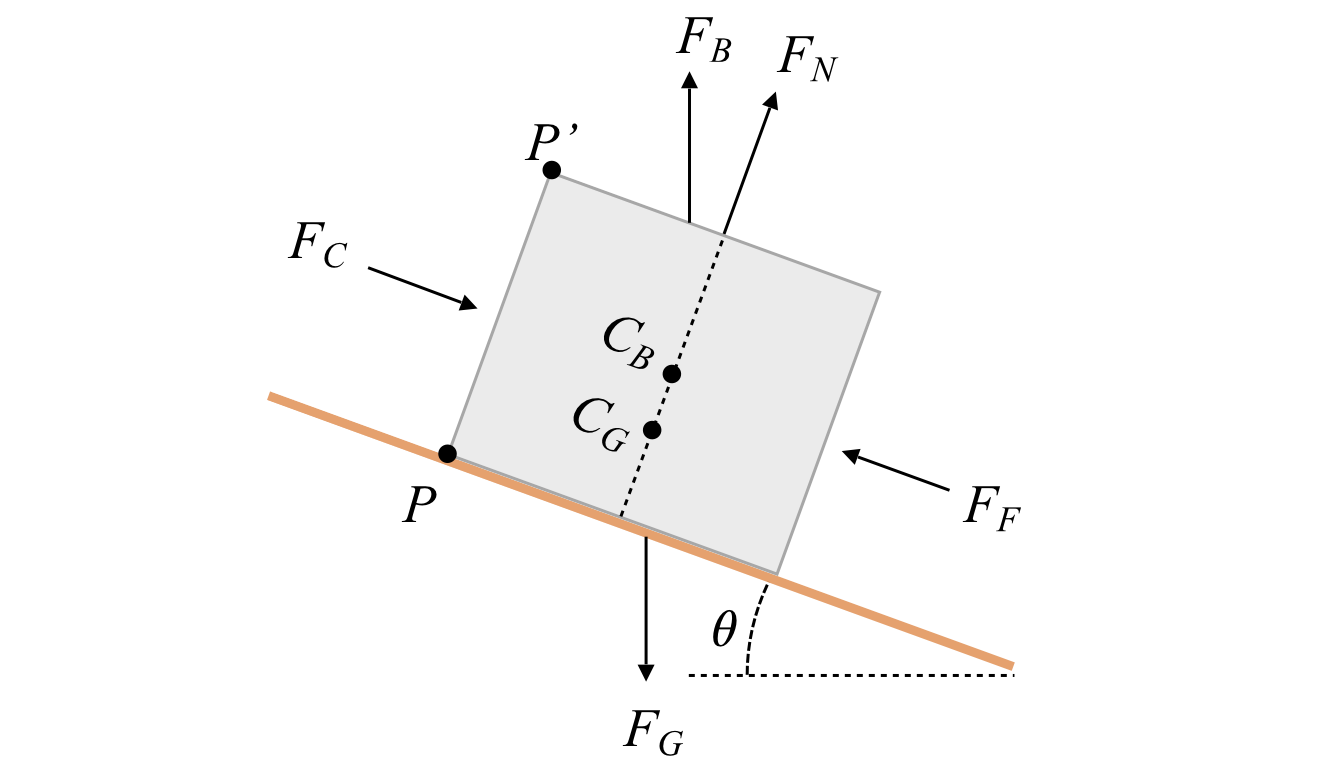
\includegraphics[width=4.8in]{./images/mehul9.png}
\caption{Forces acting on the AUV after landing on the sloping surface}
\label{f:mehul9}
\end{figure}

 Since the seafloor can have different compositions, it is difficult to estimate the exact coefficient of friction without identifying the actual nature of the seafloor. Hence, to analyze the effects of friction, current velocity values are calculated for angles between $0^\circ$ to $35^\circ$ and coefficients of friction $0.1$ and $0.6$. The values of coefficients of friction are selected based on pervious seafloor measurements ~\cite{Lambrakos1985} and seafloor currents using the Gebco database. The results indicate that the vehicle seafloor current values are within acceptable limits as seen in Fig.~\ref{f:mehul10}. 
 
\begin{figure}[!ht]
\centering
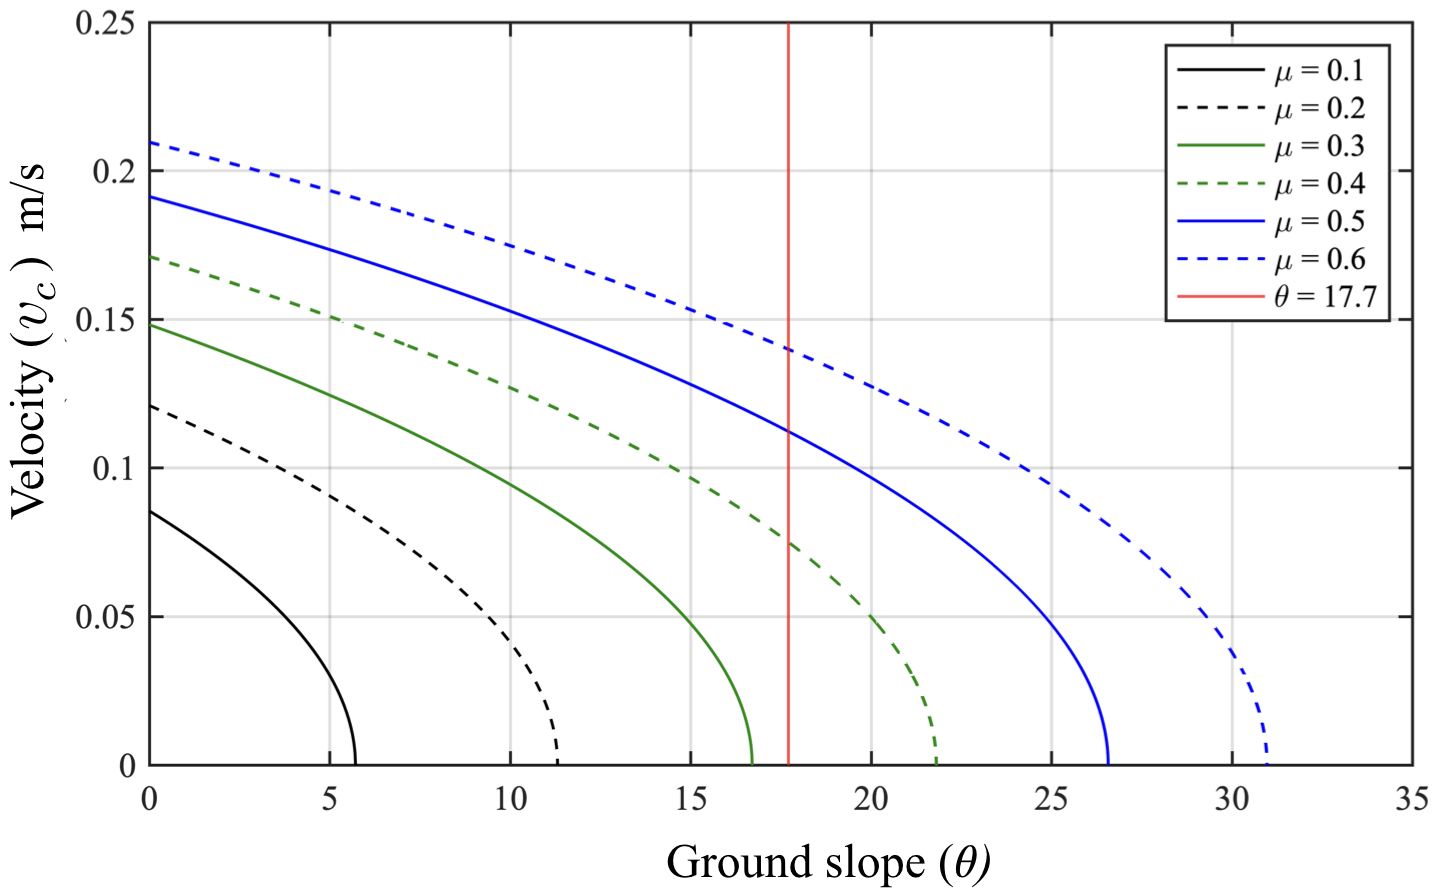
\includegraphics[width=4.5in]{./images/mehul10.png}
\caption{Analysis of seafloor currents and friction on the ground slope}
\label{f:mehul10}
\end{figure}

\subsubsection{Landing on object on the seafloor}

While landing on objects, the AUV is considered safe if the remaining part of the AUV makes full contact with the ground and is stable. Unfavorable conditions occur when the vehicle lands on an object and is partially suspended due to its righting moment. In this work, we analyze the the landing of an AUV at a point $P_i$ on the edge on an object at a distance $d_i$ from the $C_G$ of the AUV as seen in Fig~\ref{f:mehul11}a. 

\begin{figure}[!ht]
\centering
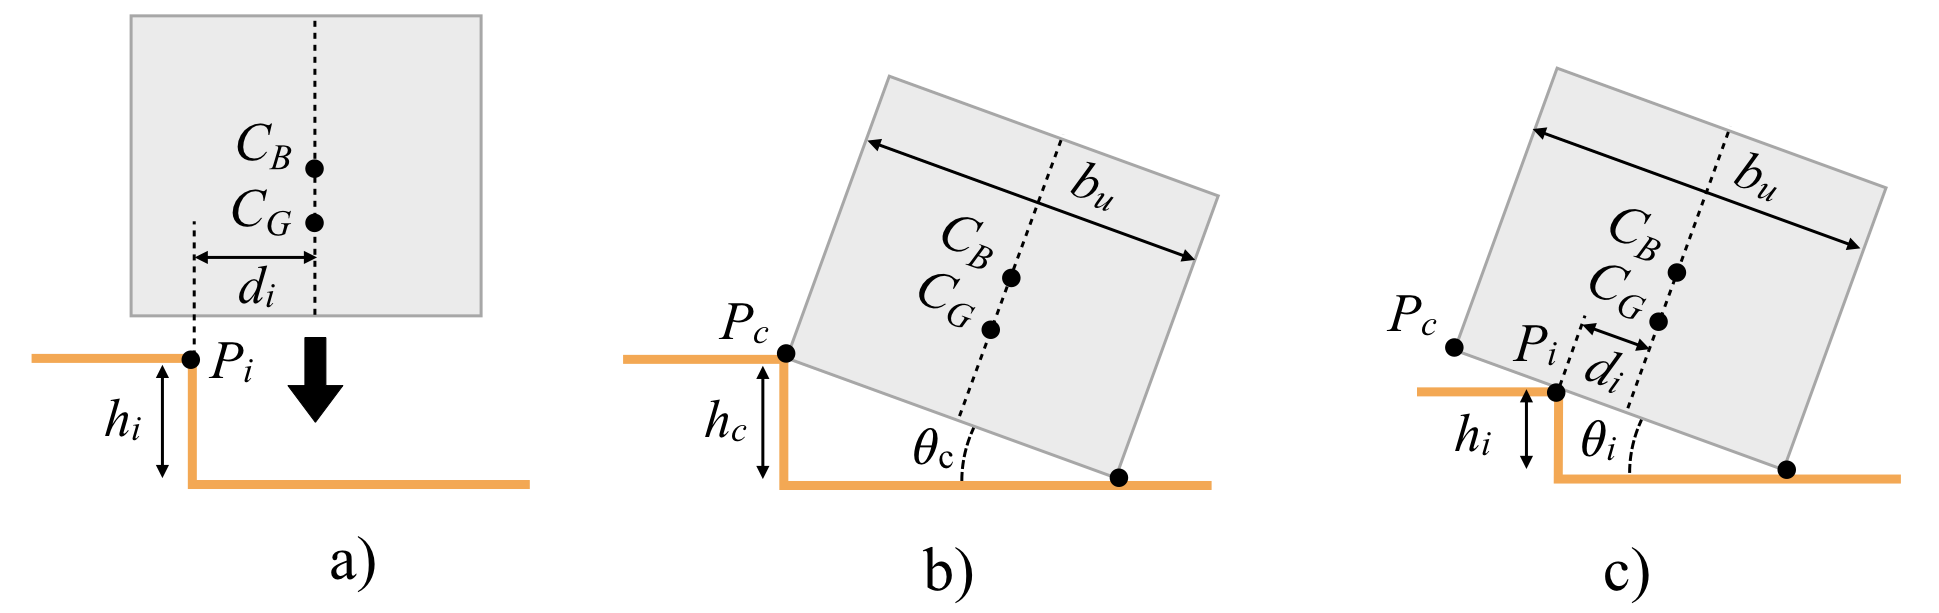
\includegraphics[width=\textwidth]{./images/mehul11.png}
\caption{a) Vehicle landing on an object on the seafloor b) Extreme condition of landing on an object c) Landing at a point between extreme condition and the centre line}
\label{f:mehul11}
\end{figure}

Extreme condition occurs when the AUV lands along its longer edge $l_u$ on the object at point $P_c$ thereby making the slope $\theta_c$ with the ground as seen in Fig~\ref{f:mehul11}b. The maximum height of the object face $h_c$ where the AUV can land safely is then calculated as:

\begin{equation}
\label{eq:eq5}
\centering
	h_c = b_u \times \sin\theta_c\
\end{equation}

The maximum height of the object face $h_c$ for our simulation is calculated as $0.152$ m. For all other points $P_i$ between $P_c$ and the $C_G$-$C_B$ centre line, we calculate the maximum angle of rotation of the AUV after making contact the object using Equation~\ref{eq:eq1} as:

\begin{equation}
\label{eq:eq6}
\centering
	\theta_i = \tan^{-1}\left[ \frac{(d_i \times F_R)}{(d_m \times F_B) - (d_g \times F_R)}\right]
\end{equation}\\

from where we can calculate the maximum height of the object face for distance $d_i$ as:

\begin{equation}
\label{eq:eq7}
\centering
	h_i = (0.5 \times b_u + d_i)\times \sin\theta_i
\end{equation}


\begin{figure}[!ht]
\centering
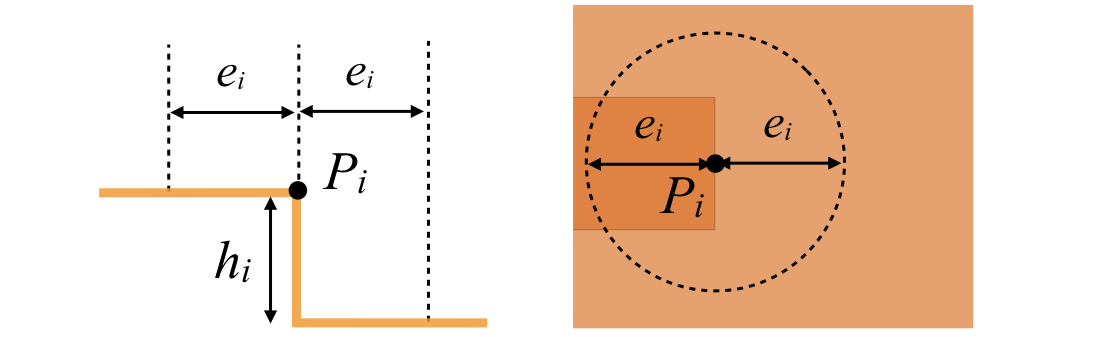
\includegraphics[width=4.5in]{./images/mehul12.png}
\caption{$C_G$ exclusion where the centre of gravity of the AUV is prohibited from landing}
\label{f:mehul12}
\end{figure}


This allows us to create a $C_G$ exclusion zone $e_i$ of size $d_i$ around each face of the object with height $h_i$ where the $C_G$ of the AUV is prohibited from landing as in Fig~\ref{f:mehul12}. The $C_G$ exclusion zone calculated in steps of $5$ mm equivalent to the mapping resolution for the dimensions of the AUV is seen in Fig~\ref{f:mehul13}.

\begin{figure}[!ht]
\centering
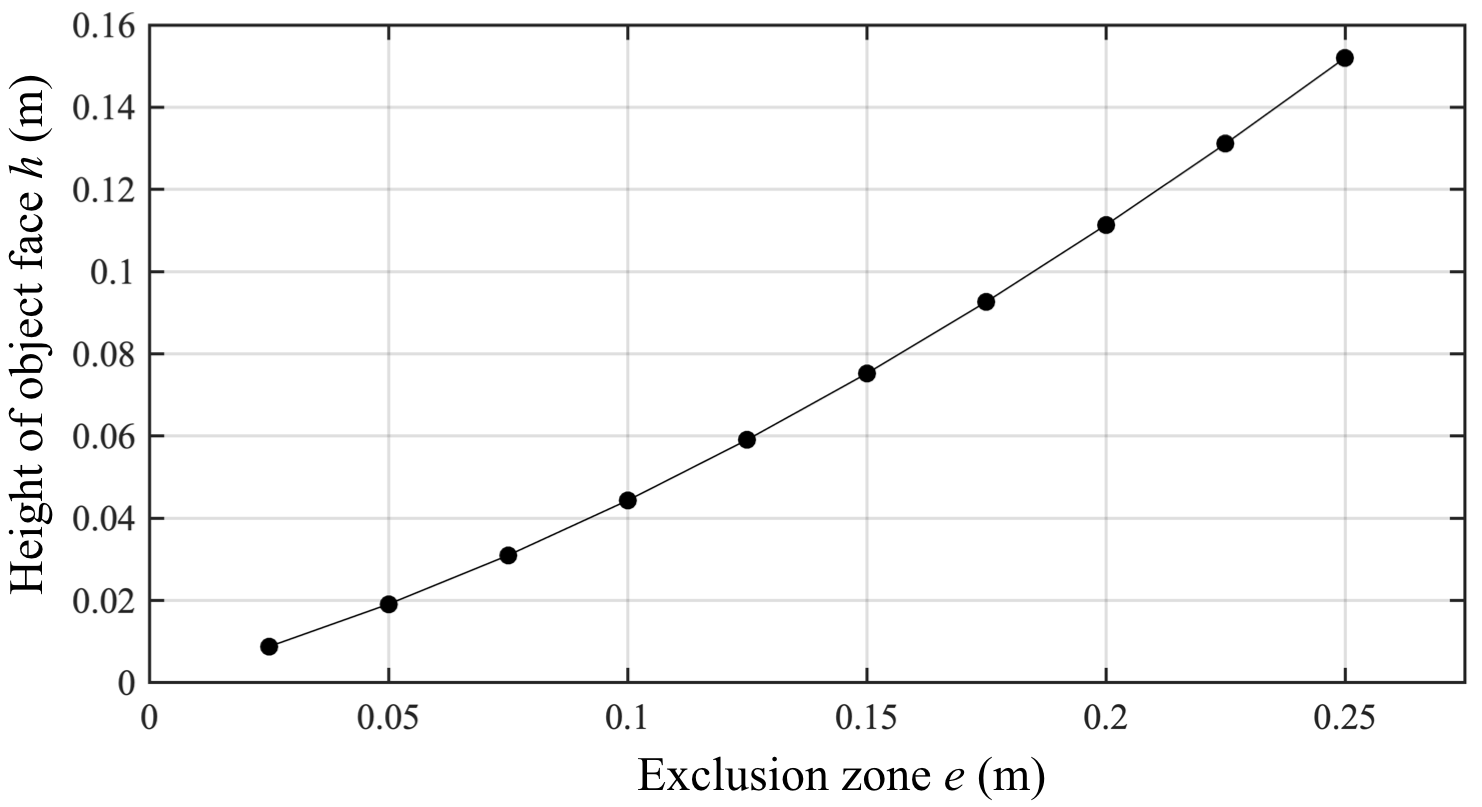
\includegraphics[width=5.5in]{./images/mehul13.png}
\caption{Exclusion zone for height of objects faces}
\label{f:mehul13}
\end{figure}

The vehicle should be prohibited from landing on object faces with height more than $h_c$ requiring a $C_G$ exclusion zone of size half the diagonal of the AUV in all directions. However, since most AUVs are not circular in shape, the $C_G$ exclusion zone for these points can be calculated based on the geometry of the AUV and the heading during landing $\alpha$. This will also reduce the size of the $C_G$ exclusion zone.  Using the conditions identified for safe landing, the flowchart of the algorithm for landing area and exclusion zone detection is seen in Fig~\ref{f:mehul14}.

\begin{figure}[!ht]
\centering
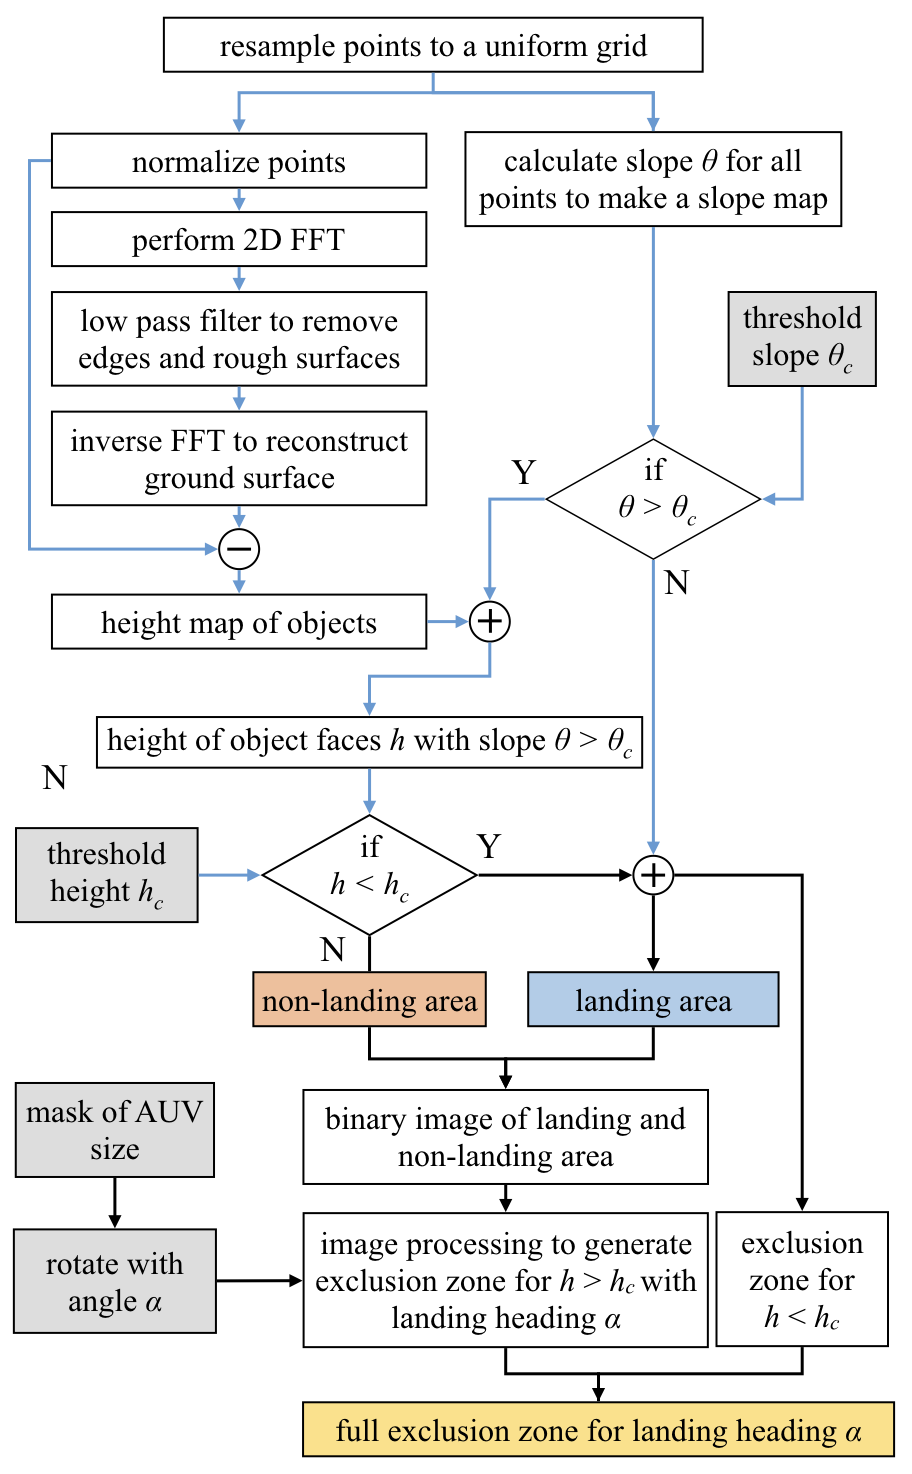
\includegraphics[width=4in]{./images/mehul14.png}
\caption{Flowchart for detection of landing area and generation of $C_G$ exclusion zone}
\label{f:mehul14}
\end{figure}

\subsubsection{Processing point cloud}


A slope map is generated for the resampled point cloud. Two vectors are computed from three neighboring points making a triangle whose cross product is taken to find the normal vector. The angle of this normal vector to the horizontal is then calculated as the slope. Slope map generated for the three areas A,B and C is seen in Fig.~\ref{f:slope_analysis}a. Slope threshold $\theta_c$ is applied to the slope map to generate a binary slope threshold map. The slope threshold map for $h_c = 17.7^\circ$ for the simulation is seen in Fig.~\ref{f:slope_analysis}b.

\begin{figure}[!ht]
\centering
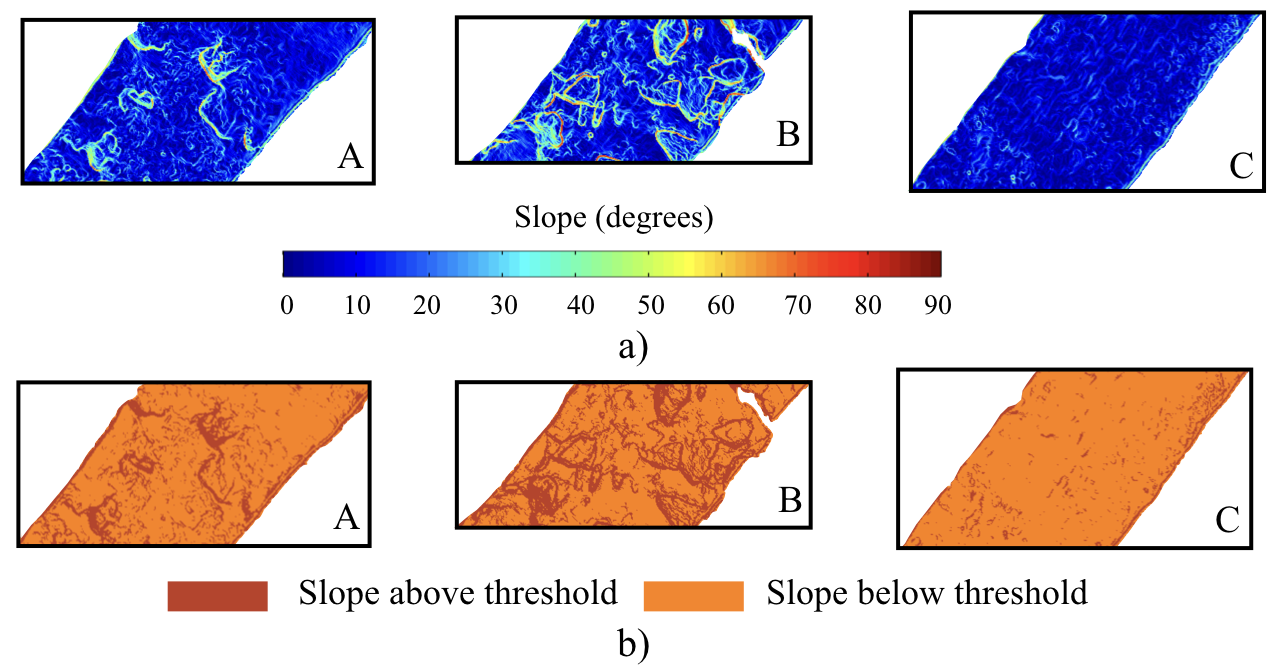
\includegraphics[width=6in]{./images/mehul15.png}
\caption{a) Slope calculated for areas A B and C. Area B shows objects having faces with higher slope than block C and A. Area C shows more smoother surface with less slope b) Slope threshold map for the three areas }
\label{f:slope_analysis}
\end{figure}

Laser projections of different seafloor terrain show distinctive profiles. The frequency content of these profiles is analyzed for separating objects from the ground surface. Flat areas are dominated by low frequency components of the profiles while the high frequency components represent the sharp edges of objects and rough surfaces. Analysis is performed on in each area using a two dimensional Fast Fourier Transform (FFT). The points in the area are zero filled on all sides to form a $N \times N$ matrix, where $N$ is the next power of $2$ more than the largest dimension of the area. The depth values of the points are then normalized to remove the DC component by subtracting the mean depth value and rotated along their Eigenvectors. Two dimensional $N$ point FFT is performed on the normalized values to convert them to frequency domain values. The frequency bins are $n \times f_s/N$, where $n = 1, 2, \dots, N/2$ and $f_s = 1/g_{res}$ the sampling frequency. A low pass filter with a linear phase response with nearly even response in the pass band and a sharp cut-off is applied to the frequency domain values to suppress the high frequency components. For cut-off frequency $f_c$, filter order $n$ and frequency bins $f$, the equation of the filter used is:

\begin{equation}
\label{eq:eq8}
\centering
	h_{l}(f) = \frac{1}{\sqrt{1 + (\frac{f}{f_c})^{2n}}} 
\end{equation}

A filter order of $3$ is used to provide suitable sharpness of damping. The filter provides a $3$ dB attenuation at the cut-off frequency. To decide the cut off frequency we identify the minimum size of the object considered as ground. For an object of size $\sigma$, represented by a step function, the equivalent sync function in frequency domain has first zero crossings at $2/\sigma$ ~\cite{Lyons1997} ~\cite{Kalogerakis2010}. The cut-off frequency is set as $f_c = 2/\sigma$ which indicates the frequency represented by the size of the object at the sampling resolution. $f_c = 5$ is used in this work. The filter function is rotated around the zero frequency to form a $N\times N$ point filter and multiplied to the frequency domain values element by element. An inverse two dimensional FFT produces smoothened values representing the ground surface. The normalized point cloud is compared to the ground surface to generate a height map of objects as seen in Fig.~\ref{f:mehul19}.

\begin{figure}[!ht]
\centering
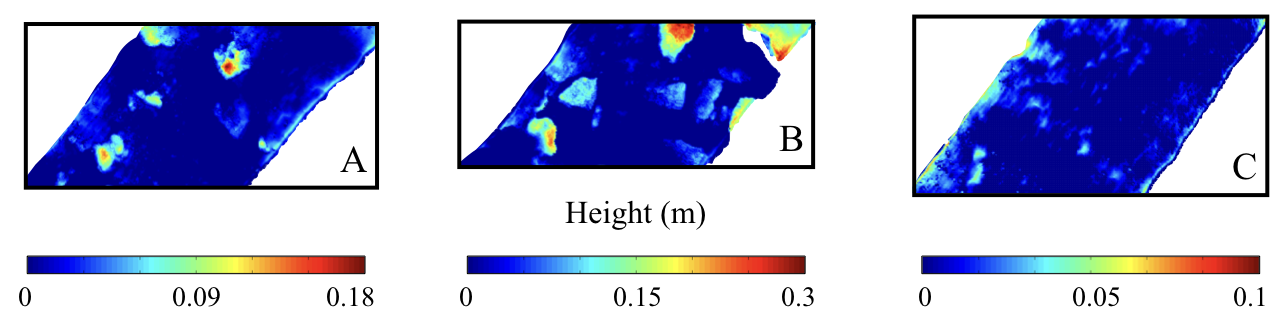
\includegraphics[width=6in]{./images/mehul19.png}
\caption{Height map for areas A B and C. Areas A and B show large objects on the seafloor compared to area C}
\label{f:mehul19}
\end{figure}

Height of object faces $h$ is extracted in areas above the slope threshold $\theta > \theta_c$ from the height map of objects as in Fig.~\ref{f:mehul20}b. A $C_G$ exclusion zone is generated for object faces with height less than height threshold $h < h_c$, using values calculated from Equation~\ref{eq:eq6} and~\ref{eq:eq7} and shown in Fig.~\ref{f:mehul13}. For this, location of all points having a certain height range are identified to form a binary image. Morphological dilation is then performed on this binary image using a circular structural element with radius equal to size of the exclusion zone for that height. Object faces with height above the threshold $h > h_c$ are identified to make a binary image with non-landing and landing area. Landing area identified for height threshold of $0.152$ m is seen in Fig.~\ref{f:mehul21}a. Since the AUV can land along different headings, the $C_G$ exclusion zone for object faces above height threshold is made taking into account the landing heading $\alpha$ and the geometry of the AUV. For this, a rectangular structural with dimensions in pixels equal to the size of the AUV is generated. The structural element is then rotated to the landing heading to generate a new structural element representing the rotated AUV.


\begin{figure}[!ht]
\centering
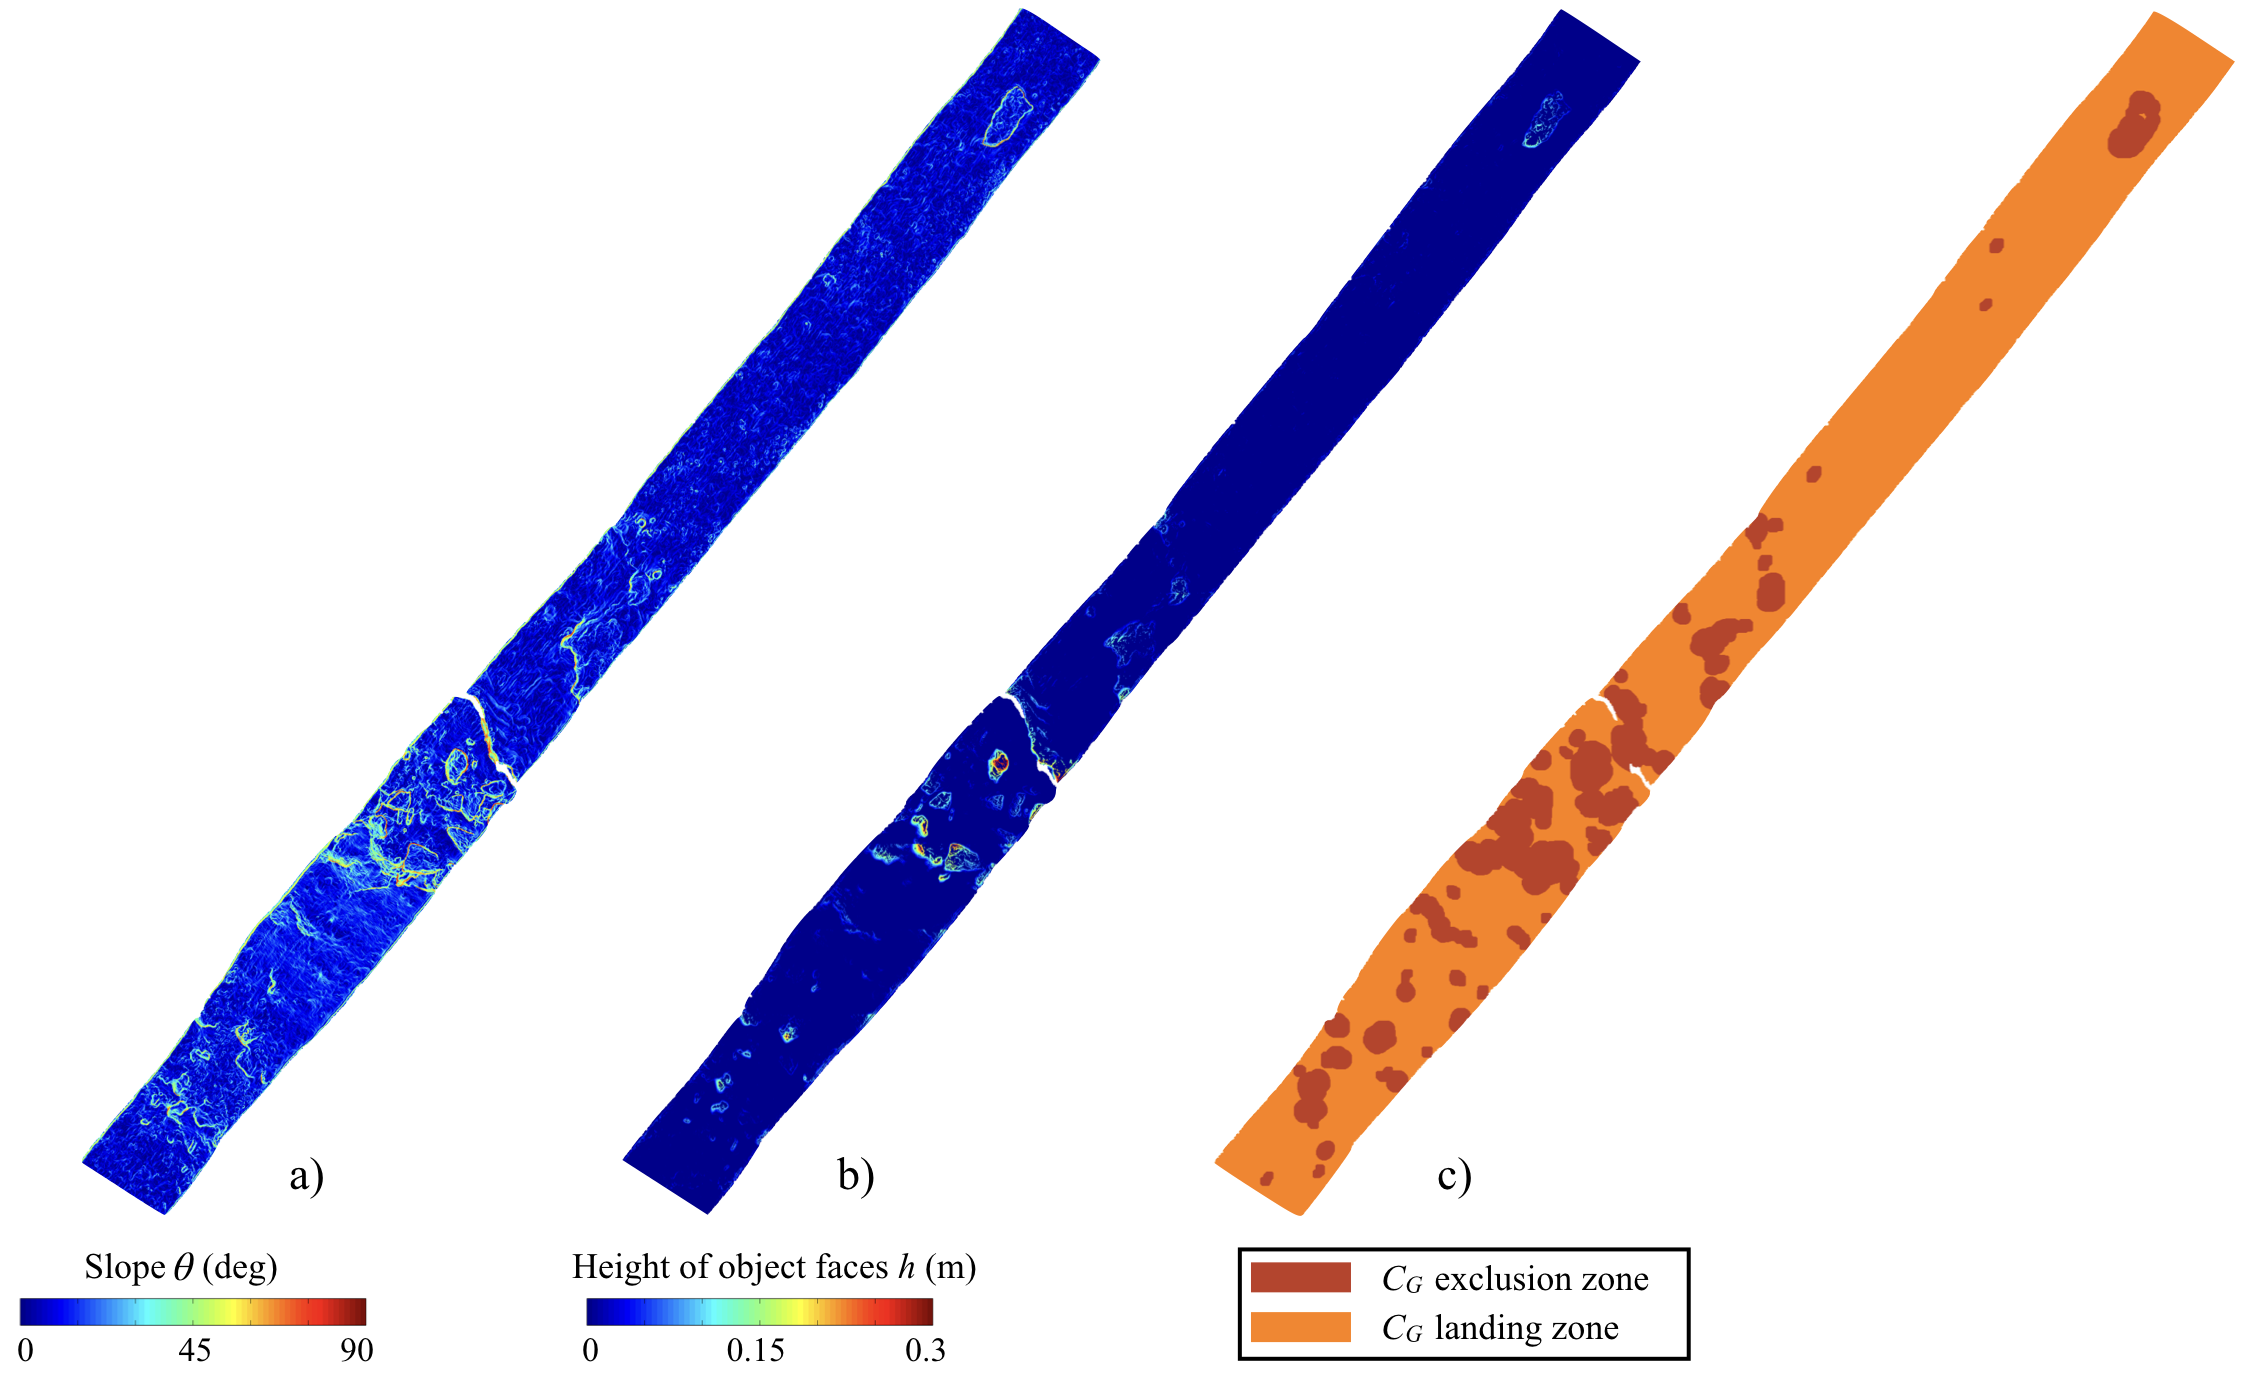
\includegraphics[width=5.5in]{./images/mehul20.png}
\caption{a) Slope map of the mapped bathymetry b) Height of object faces $h$ for slope $\theta > \theta_c$ c) $C_G$ exclusion zone for object faces $h < h_c$}
\label{f:mehul20}
\end{figure}

\begin{figure}[!ht]
\centering
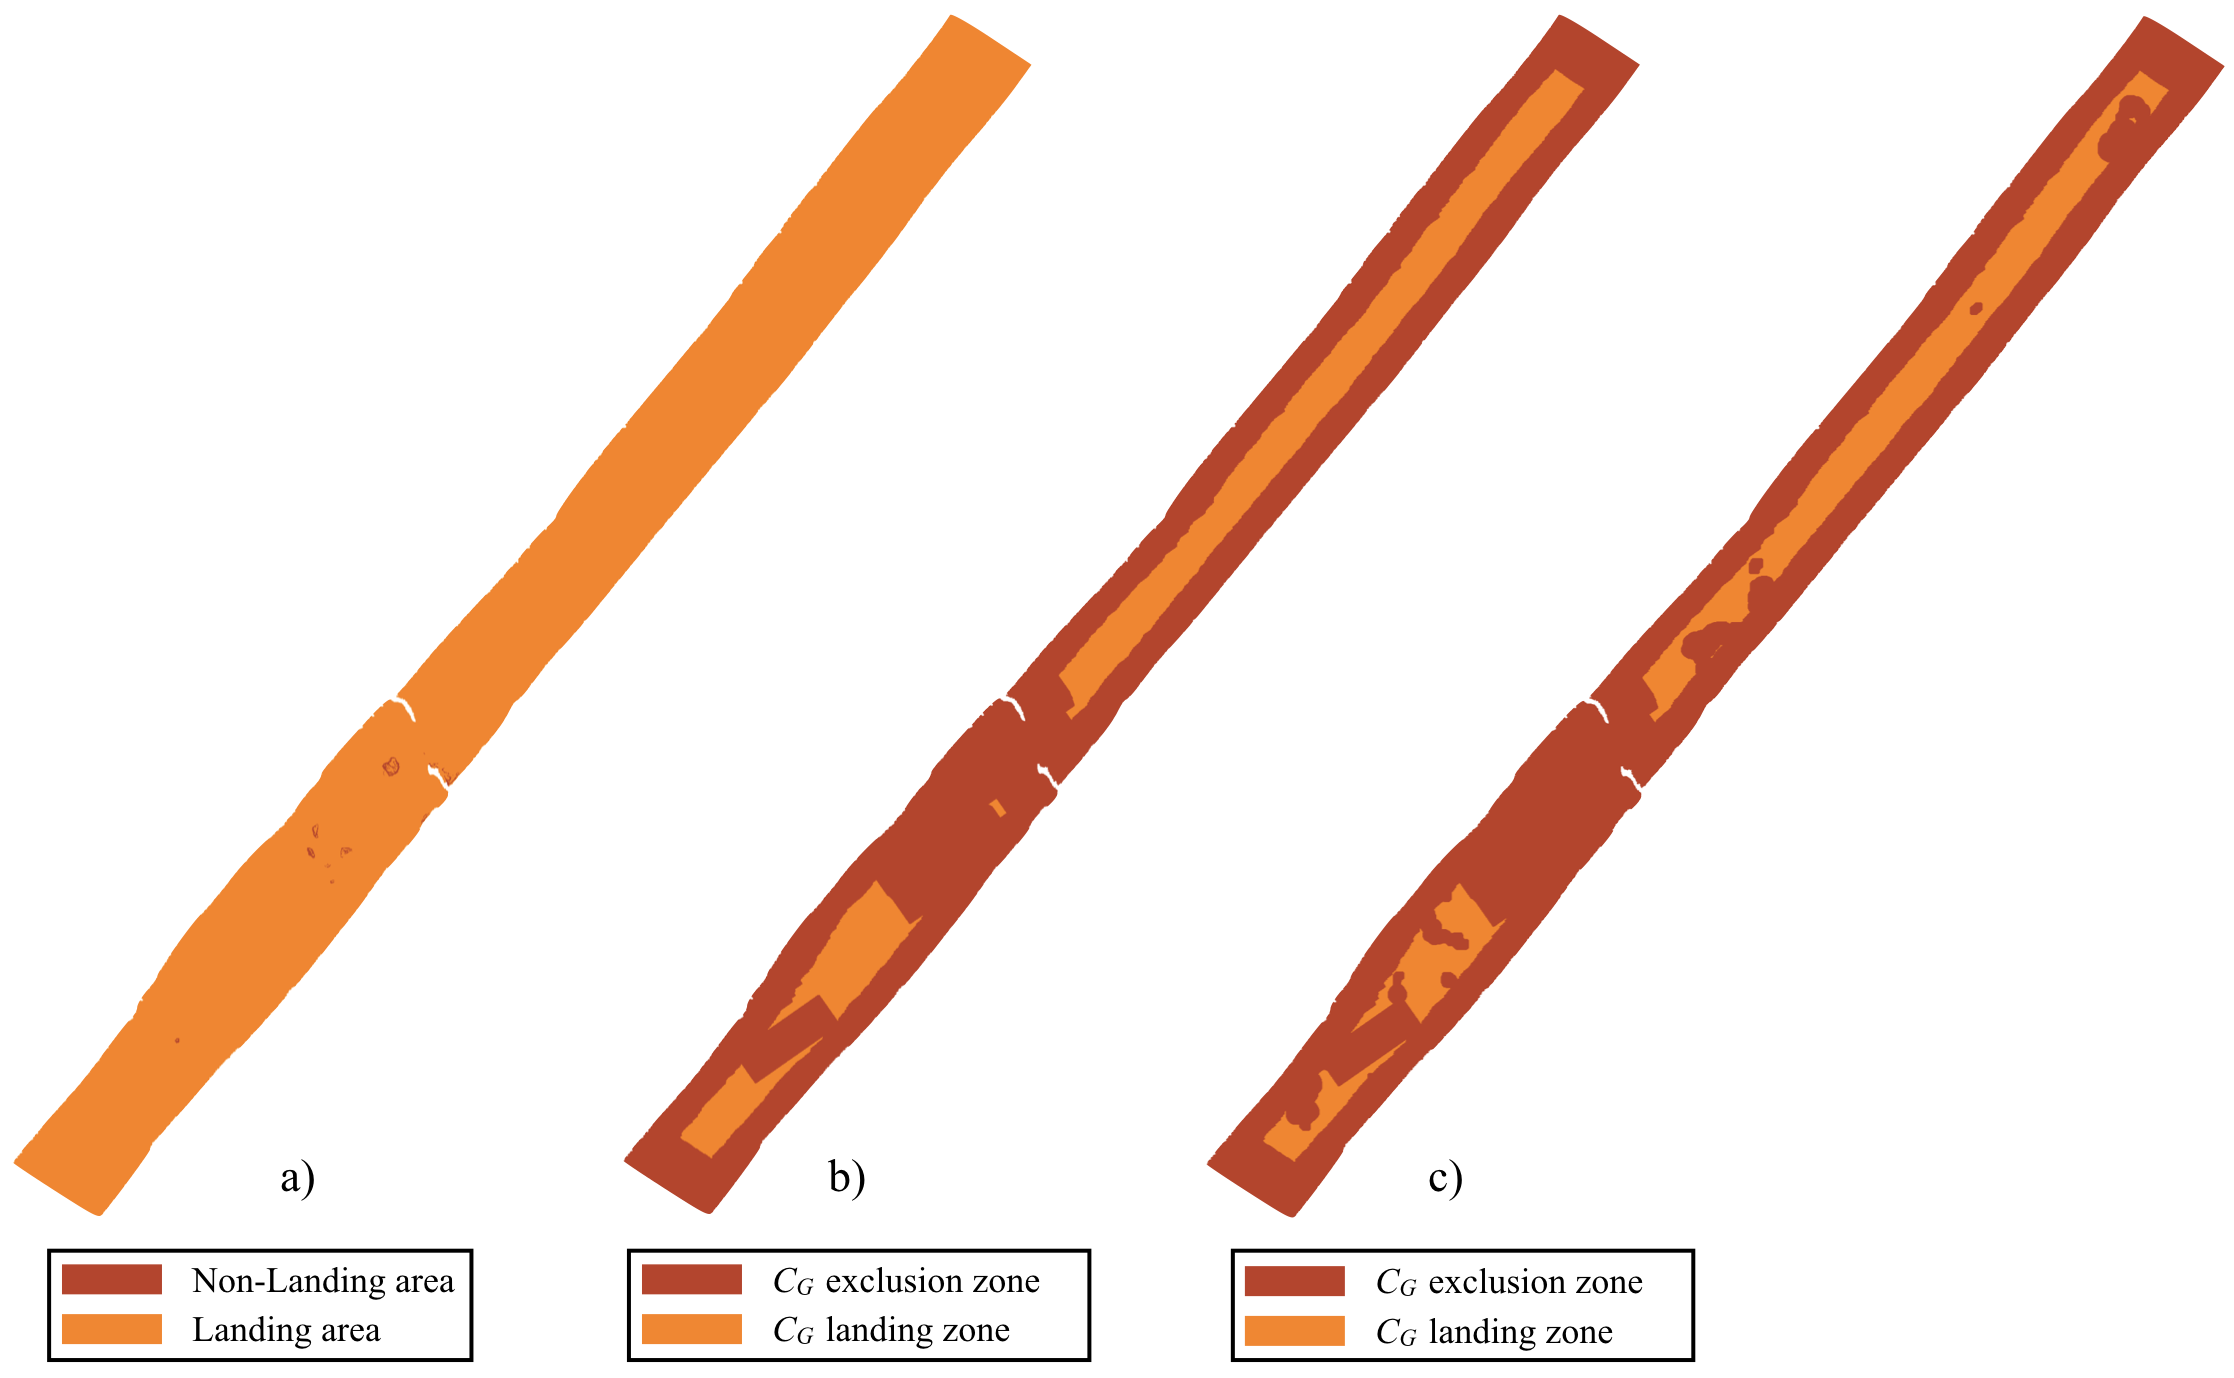
\includegraphics[width=5.5in]{./images/mehul21.png}
\caption{a) Landing area for height threshold $h > h_c$ b)  $C_G$ Exclusion zone for landing area with $55^\circ$ landing heading  c) Full $C_G$ exclusion zone for object faces $h < h_c$ and landing area with $55^\circ$ landing heading}
\label{f:mehul21}
\end{figure}

 Image opening is performed between the rotated structural element and the binary image to find area where the AUV can fit in the landing area. The points are further eroded using the rotated structural element to find area where the $C_G$ of the AUV can land. The remaining are marked as  $C_G$ exclusion zone for the landing heading. $C_G$ exclusion zone for a landing heading of $55^\circ$ is as seen in Fig~\ref{f:mehul21}b. This exclusion zone is then combined with that generated for object faces with height less than height threshold $h < h_c$ to make a full $C_G$ exclusion zone as seen in Fig~\ref{f:mehul21}c. 
 
\subsection{Identifying landing sites}

Landing sites are identified where the AUV can fit and safely land along a landing heading. For each heading, area other than the $C_G$ exclusion zone, $C_G$  landing zone is split into grounds based on eight neighboring connected pixels. Each group is identified as a landing site. The three landing sites identified for the landing heading of $55^\circ$ can be seen in Fig~\ref{f:mehul22}a.

\begin{figure}[!ht]
\centering
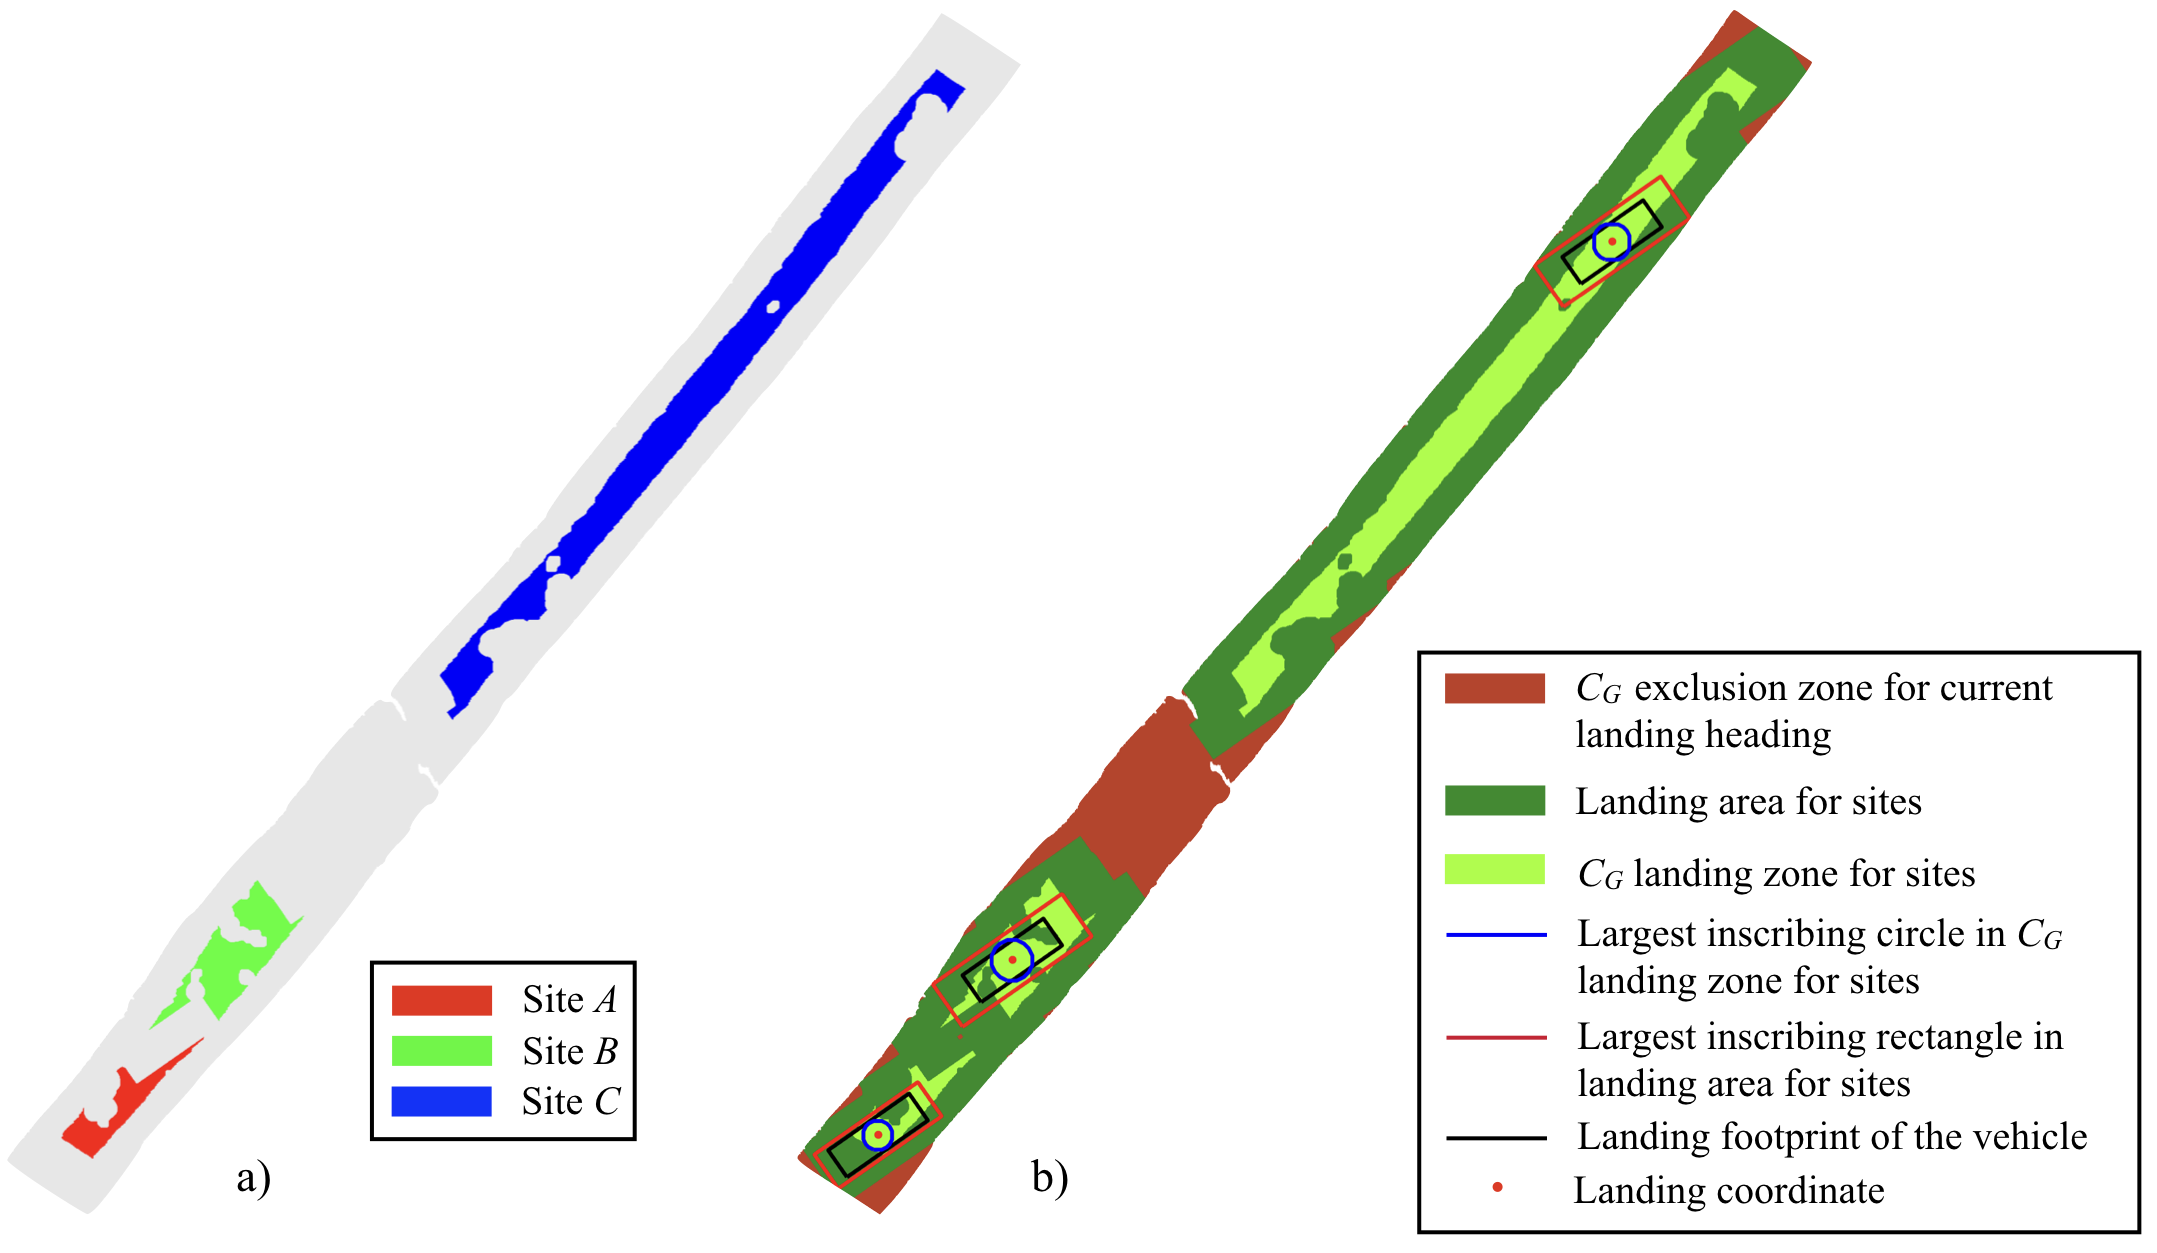
\includegraphics[width=6in]{./images/mehul22.png}
\caption{a) Landing sites identified for $55^\circ$ landing heading  b) Landing point calculation }
\label{f:mehul22}
\end{figure}

	Small groups of points are rejected since the are too small for the AUV to 
	relocate and navigate for landing due to positioning errors. A landing 
	coordinate is calculated for each site where the AUV can land furthest away 
	from the boundary of the site. For this, the largest circle that can be 
	inscribed in the site is calculated and centre of this circle is taken as 
	the landing coordinate. The footprint of the vehicle around the landing 
	coordinate along the landing heading is generated to form a rectangle where 
	the properties of the landing site are extracted. The landing coordinates 
	calculated for the site along landing heading of $55^\circ$ are seen in 
	Fig~\ref{f:mehul22}b. The following properties of the landing site are 
	extracted:\\
	
\subsubsection{Site slope $P_s$}  The mean landing slope $\overline{\theta}$ is calculated for the points in the landing footprint of the AUV. The slope is then normalized using the threshold slope $\theta_c$ to get the value of $P_s$: 
	
\begin{equation}
\label{eq:eq9}
\centering
	P_s = \frac{\overline{\theta}}{\theta_c}
\end{equation}
	
\subsubsection{Site safety $P_f$} A safety factor is calculated for the landing point which indicated how far the vehicle is from the edges of the landing site. For each site, the landing area for that site is calculated by morphological dilation of the site using the rotated structural element. The largest rectangle around the landing coordinate that can be inscribed within this landing area having same aspect ratio and landing heading as the vehicle is calculated. The ratio of area of this rectangle $A_r$ to the footprint of the vehicle $A_f$ is calculated as a safety ratio. Since values above a certain limit do not provide any additional safety, the safety ratio is limited to $5$. The value of $P_f$ is then calculates as:

 \begin{equation}
 \label{eq:eq10}
    P_f = \frac{1}{4}\left( 5 - \frac{A_r}{A_f}\right) 
  \end{equation}
	
 \subsubsection{Site roughness $P_r$} Roughness value $R$ is calculated for area under the the vehicle footprint as the average deviation of the height values $h$ from the mean $\overline{h}$. This value is then normalized by comparing with the maximum possible roughness for any terrain under the vehicle footprint $R_m$. Since the landing coordinate is not included in the $C_G$ exclusion zone, the worst case scenario of the height map is as seen in Fig.~\ref{f:mehul22a}. The roughness calculated for this is $R_m = 0.03$.

\begin{equation}
 \label{eq:eq11}
	R = \frac{1}{n} \sum_{i=1}^{n}\left | h_i - \overline{h} \right |
\end{equation} 

\begin{equation}
 \label{eq:eq12}
	P_f = \frac{R}{R_m} 
\end{equation}\\ 

\begin{figure}[!ht]
\centering
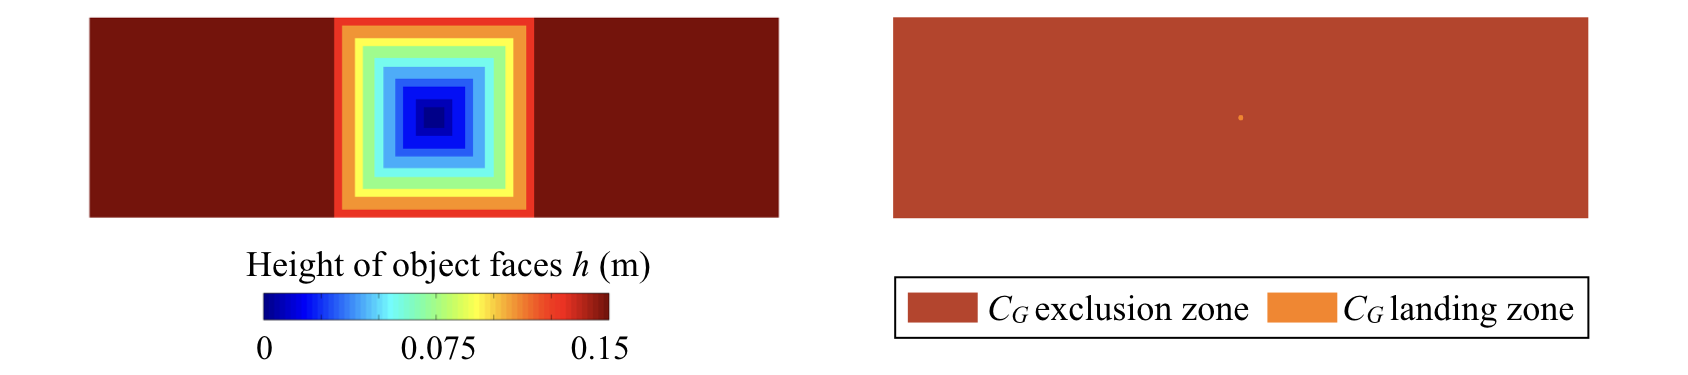
\includegraphics[width=6in]{./images/mehul22a.png}
\caption{Area equal to the landing footprint of the vehicle with possible height values with the centre as landing zone}
\label{f:mehul22a}
\end{figure}
 
 Landing cost $C_s$ is calculated for each site as the average of the three extracted site properties:
 
 \begin{equation}
 \label{eq:eq13}
	C_s = \frac{1}{3}\left[P_s + P_f + P_r \right]
\end{equation} 

Landing costs calculated for the three sites for landing heading $55^\circ$ are seen in Table~\ref{t:table4}. The final landing site for this heading is selected as the one with least landing cost, in this case site C.
   			
\begin{table}[!ht]
\centering
\caption{Landing site properties}
\begin{tabular}{  |p{2cm} p{2cm} p{2cm} p{2cm} p{2cm}| }
\hline
\textbf{Site} & \textbf{$P_s$} & \textbf{$P_f$} & \textbf{$P_r$} & \textbf{$C_s$}\\ \hline 
$A$ & $0.54$ & $0.85$ & $0.29$ & $0.56$ \\
$B$ & $0.67$ & $0.62$ & $0.32$ & $0.54$ \\
$C$ & $0.34$ & $0.65$ & $0.15$ & $0.38$ \\
\hline
\end{tabular}
\label{t:table4}
\end{table}

\subsection{Selecting final landing site}

To select a final landing site for the mapped bathymetry, we need to analyze landing sites along different landing headings. The landing site with the least landing cost can be along any landing heading depending on the vehicle geometry and the seafloor terrain. Landing sites are identified for landing headings between $-90^\circ$ and $90^\circ$ in steps of $5^\circ$. Landing sites along the opposite headings are identical due to the rectangular nature of the structural element. The landing costs calculated for all the landing candidates are seen in Fig.~\ref{f:mehul23}. The landing site $B$ for landing heading $40^\circ$ has the least landing cost and selected as the final landing candidate. The properties for final landing candidate are as in Table ~\ref{t:table5}.


\begin{figure}[!ht]
\centering
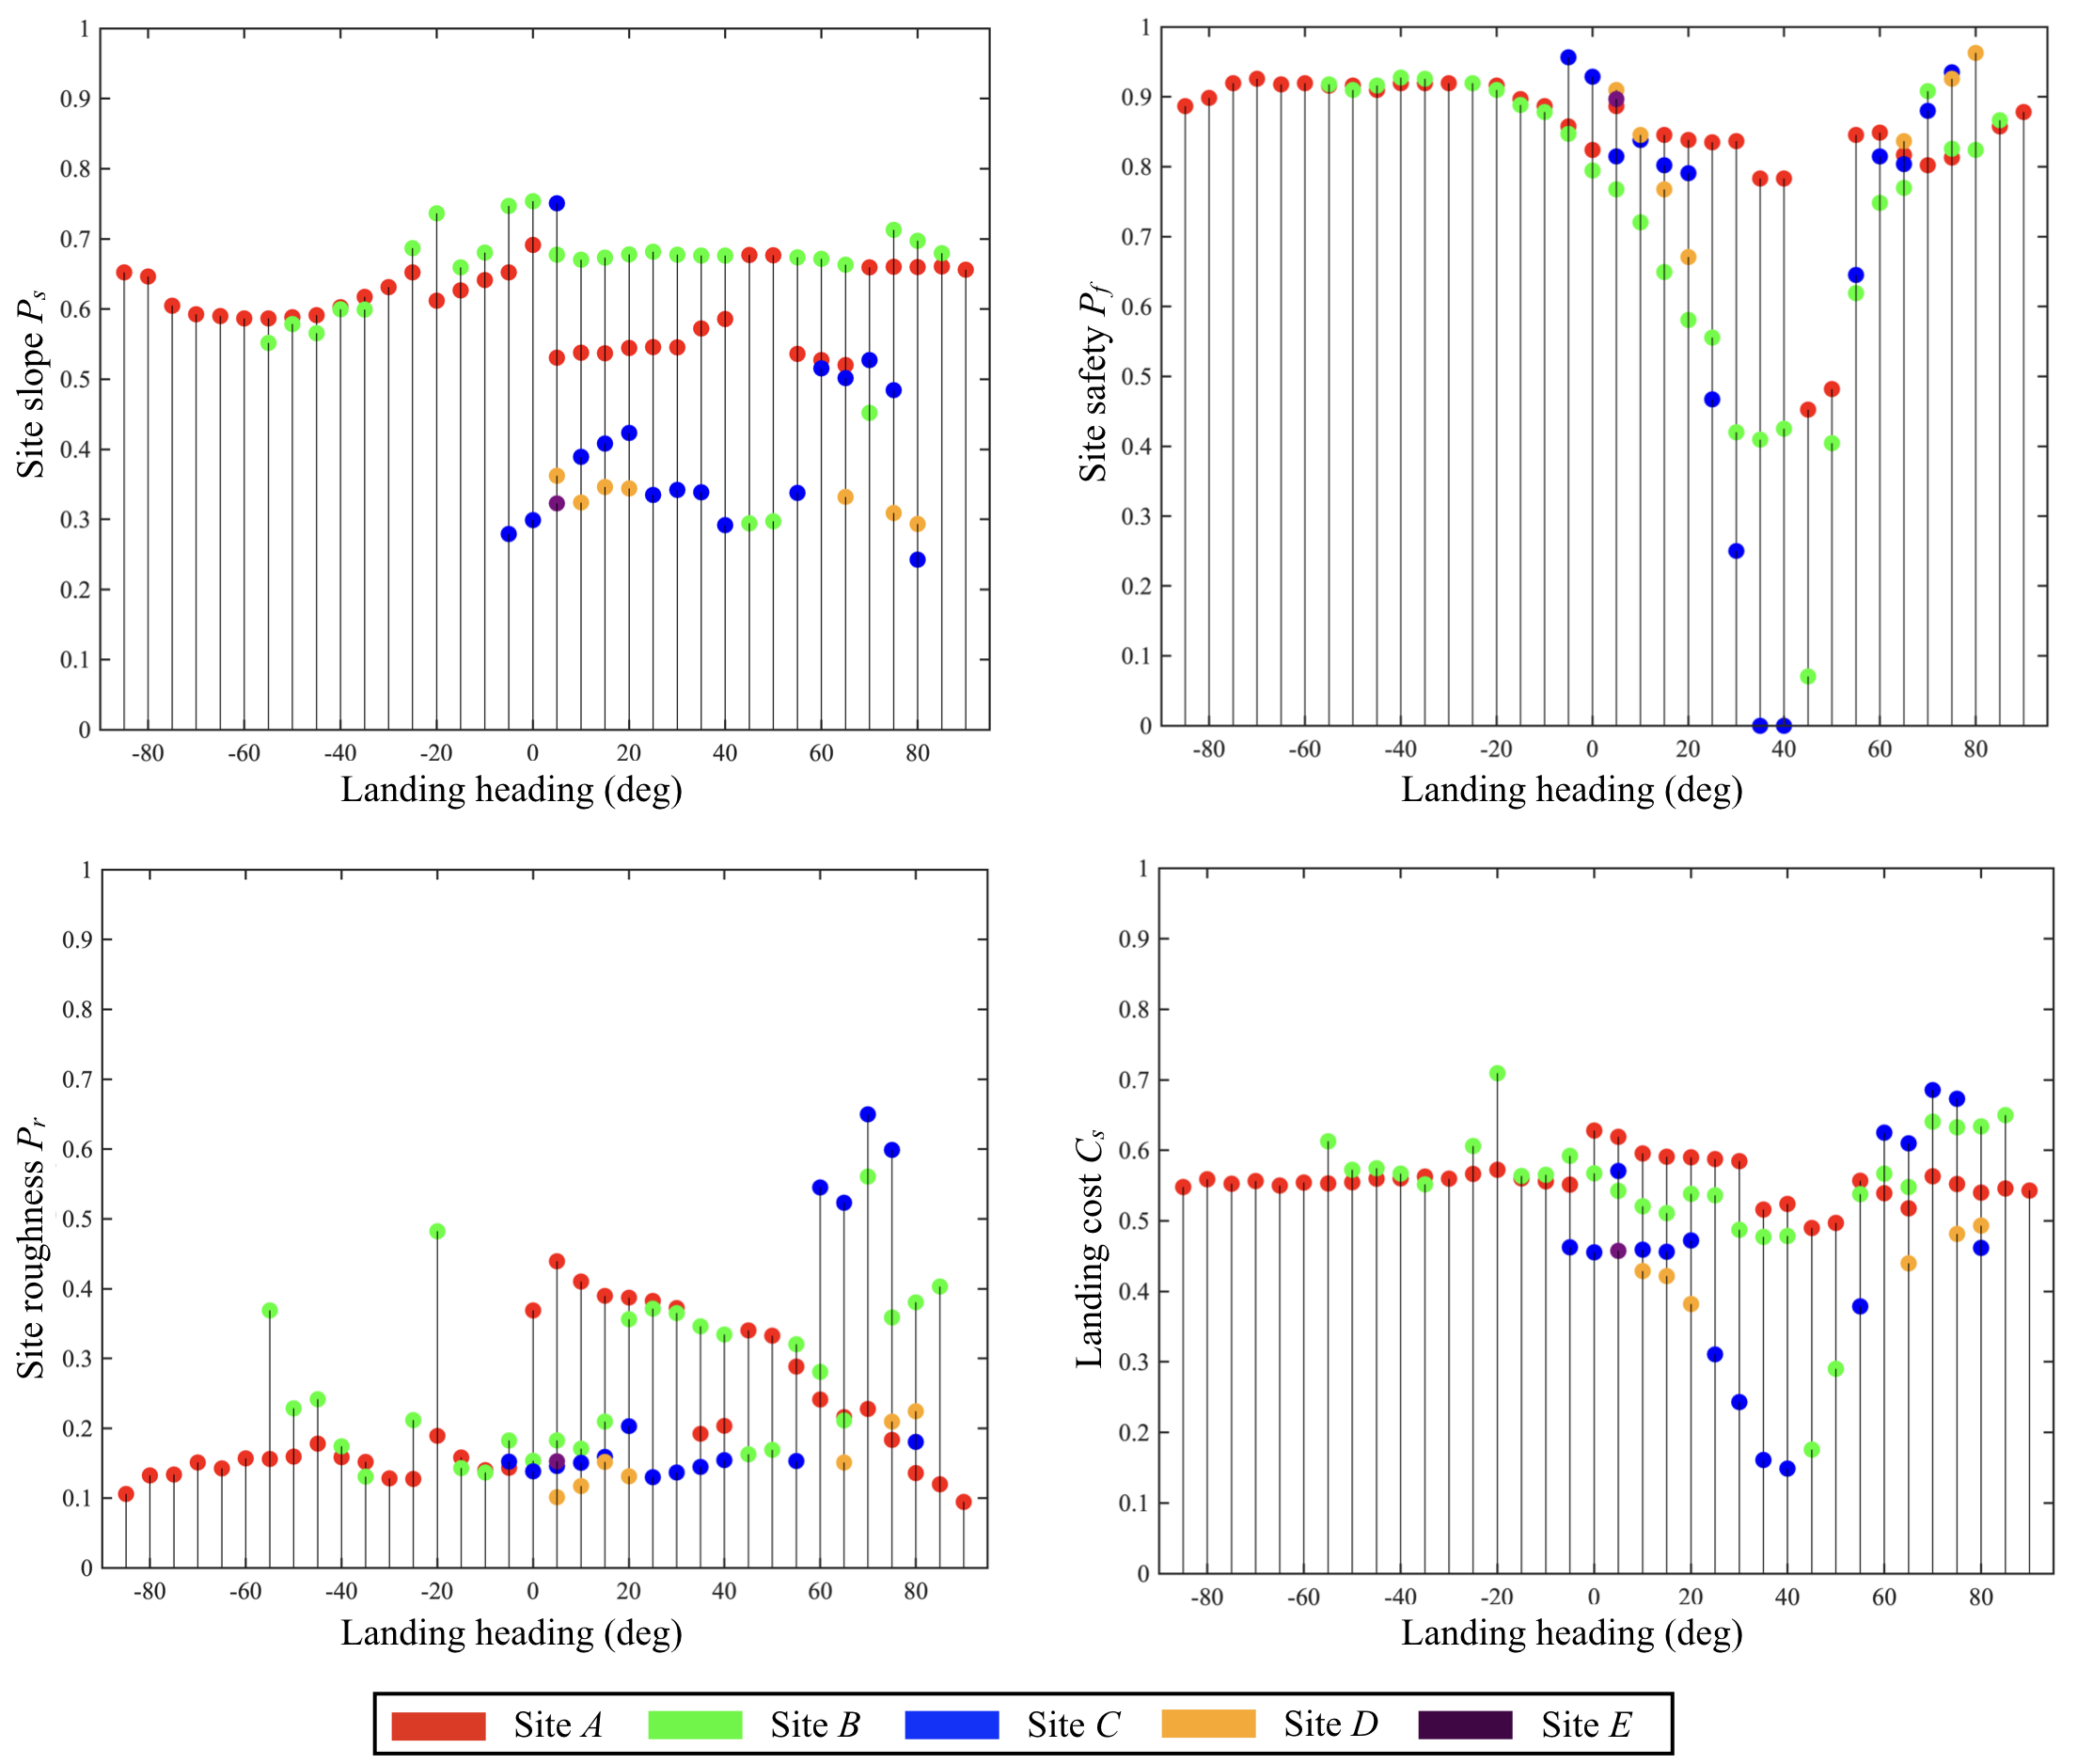
\includegraphics[width=\textwidth]{./images/mehul23.png}
\caption{Properties of the landing sites}
\label{f:mehul23}
\end{figure}


\begin{table}[!ht]
\centering
\caption{Properties for final landing site}
\begin{tabular}{  |p{6cm}  p{4cm}| }
\hline
\textbf{Property} & \textbf{Value}\\ \hline 
Landing heading & $40^\circ$ or $220^\circ$ \\
Mean depth & $1379.72$ m\\
$P_s$ & $0.29$\\
$P_f$ & $0.00$\\
$P_r$ & $0.16$\\
$C_s$ & $0.15$\\
\hline
\end{tabular}
\label{t:table5}
\end{table}
